\documentclass[12pt, a4paper]{book} %Esboco_Tese_Doutorado_2023-09-20
%\documentclass[tese]{abntex2} %Alternativa de tipo de documento (nesse caso, consultar documentação do pacote abntex2)
\usepackage[utf8]{inputenc} %Codificação
\usepackage[brazilian]{babel} %Idioma do documento e ortografia geral
\usepackage[alf]{abntex2cite}
\usepackage{setspace} %Espaçamento de linhas
\usepackage{graphicx} %imagens
\usepackage[hycap]{caption} %legenda
    %\captionsetup[figure]{labelsep=none} %formato legenda
    \usepackage{chngcntr} %fazer contagem global das figuras
        \counterwithout{figure}{chapter} %fazer contagem global das figuras
\usepackage[colorlinks=true, allcolors=blue]{hyperref} %referência cruzada
    \renewcommand{\thefigure}{\arabic{figure}}
\usepackage{xcolor} %cor da fonte
    \definecolor{textcolor}{RGB}{56,74,103} %cor fonte livro Waldheim
    \definecolor{labelcolor}{RGB}{96,86,78} %cor legenda livro Waldheim
\usepackage{tcolorbox} %caixa de texto
%%%%%%%%%%%%%%%%%%%%%%%%%%%%%%%%%%%%%%%%%%%%%%%%%%%%%%%%%%%%%%%%%%%%%%%%%%
\begin{document}

\frontmatter % Seção de pré-texto (capa, sumário, resumo, etc.)

% Title Page
\title{Traçados Urbanos 

Morfologicamente Adequados:

Diretrizes de Projeto}

\author{Higor Ribeiro da Costa}
\date{Maringá, 2023}

    \maketitle

    \tableofcontents
    \listoffigures %Lista de figuras
    \listoftables %Lista de tabelas

    %\input{resumo} %Arquivo com o resumo da tese

    \mainmatter % Corpo principal da tese

    \onehalfspacing
    

    \part*{}

        \chapter*{Introdução}
        \addcontentsline{toc}{chapter}{Introdução}
        
        Há muito que me pergunto o porquê de nossas cidades serem tão `feias', e penso que isso tenha que ver com seus traçados. Talvez `feio' não seja o melhor termo para descrever esse aspecto da realidade, pois não se trata aqui de um mero juízo estético de minha parte. Porém, ``enquanto tem-se dificuldade para encontrar um parâmetro conjunto para o [termo] `belo', em relação ao [termo] `feio' parece ser menos problemático encontrar um terreno comum'' (Daverio, 2022, \textit{s.p.}, tradução nossa).
            \footnote[1]{\textit{``mentre sul bello si fatica a trovare un parametro congiunto, sul brutto sembra essere meno problematico trovare un terreno comune''} (Daverio, 2022, \textit{s.p.}.} 
        `Se hoje temos tanta tecnologia, por que fazemos casas e prédios, mas, sobretudo, bairros e cidades assim?' Assim `desconjuntados', que `não fazem sentido.' Por que os loteamentos parecem `arranhões de gato' sobre as colinas, com ruas tão íngremes que não permitem a caminhada, dificultam o acesso do transporte, e promovem enxurradas que levam as casas para dentro dos rios? Essa foi uma dúvida que me perseguiu por anos, e, ao começar a entender as causas desse fenômeno, pesquisar uma solução – ou pelo menos uma alternativa – pareceu-me imprescindível.

        $<$FIGURA COM LOTEAMENTO DO TIPO `ARRANHÃO DE GATO'$>$

        É necessário salientar que entre o campo da edilícia e o da cidade há uma lacuna considerável. Quero dizer, quando falo em arquitetura `feia,' quero significar aquela arquitetura que não é orgânica – \textit{i.e.,} cujas partes não são interdependentes – e que não tem uma relação com seu contexto espaço-temporal. Ou seja, uma arquitetura que não conecta passado e futuro em si própria – em termos de soluções técnicas, organizativas, formais, etc. E explicações para esse fenômeno não nos faltam (Caniggia e Maffei, 2008 [1979]; Strappa, 1995).

        Porém, para as cidades já não temos tantas explicações – talvez, precisamente, pela complexidade do tema. O que é uma cidade `feia'? É apenas uma cidade inorgânica? Uma cidade cujo traçado não tem relação com seu contexto – tanto natural como antrópico? E o que fez as cidades se tornarem assim? Ou, em resumo, o que faz com que as novas áreas urbanas tenham, não raro, uma qualidade inferior a antigas áreas urbanas? É certo que vemos as benesses das infraestruturas que não existiam no passado, no entanto, por exemplo, as áreas históricas de cidades antigas fazem os olhos de turistas – ainda que atraídos pelo marketing, mas marketing que soube evidenciar as características positivas de tais áreas. E que características seriam essas? Posso apontar duas, pelo menos. A primeira é a coerência entre as edificações da área, não raro em um \textit{continuum} de fachadas que cria um grande cenário urbano – cenário autêntico. E a segunda é a conformação do traçado que lhes dá suporte, com todos os seus elementos – e isso é o que me interessa.

        \begin{center}
        . . . . .
        \end{center}

        No fim de minha dissertação de mestrado, cheguei à conclusão de que é possível projetar traçados urbanos morfologicamente adequados ao contexto. E explico o que quero dizer com isso. `Contexto' aqui é o conjunto de estruturas naturais e antrópicas de uma área com suas respectivas características. `Morfologicamente adequado' quer dizer aquilo que já é, desde sua concepção, coerente com o formato das estruturas do contexto dado pela realidade. E traçado urbano é a marca das estruturas urbanas que o homem desenvolve.

        No caso das estruturas naturais, o que tomo por mais importante é a orografia, a terra com a sua forma, que é sobre onde se assentam as estruturas que o homem desenvolve, seguida pela hidrografia. Uma área pode ser mais íngreme ou suave, mais ou menos extensa, e seu relevo possui uma hierarquia latente, que pode ser destrinchada por meio de cumeadas, pontos de distribuição, assim como por talvegues e pontos de encontro. E, no caso das estruturas antrópicas, temos parcelamentos rurais precedentes, franjas urbanas com loteamentos, e diretrizes viárias. Com isso, temos ruas e avenidas, lotes urbanos e glebas rurais com seus limites. Cada uma dessas estruturas naturais e antrópicas desenvolve uma relação de interdependência, existencial – pois algumas não podem existir sem outras – e morfológica, por meio de seus formatos poligonais e consequentes angulações – bidimensional ou tridimensionalmente. 

        Ou seja, quando digo que um traçado urbano deve ser `morfologicamente adequado ao contexto', quero implicar que cada um de seus elementos (sobretudo ruas, praças, demais espaços abertos, e os lotes e quarteirões que derivam de sua disposição) deve, na máxima medida possível, seguir, primeiro, os formatos dados pela estruturação natural e, segundo, os formatos dados pelos elementos da estruturação antrópica. E isso se opõe ao \textit{laissez-faire} dos traçados concebidos \textit{a priori} e só depois `adaptados' à realidade, que se impõe forçosamente ao projetista contrariado. Um traçado `adequado' é diferente de um traçado `adaptado'. É a morfogênese planejada contraposta ao automatismo.

        \begin{center}
        . . . . .
        \end{center}

        Durante aquela pesquisa, da qual a presente tese não é senão o desdobramento, desenvolvi o conceito de `\textit{rendimento} urbano' – que afirma que deve existir uma ``coerência intrínseca'' entre o traçado urbano e o contexto natural (Costa e Rego, 2019, p. 7); e projetei um traçado urbano hipotético sobre uma área urbana consolidada, comparando-o com o traçado existente e com a legislação local em vigor. Com isso, verifiquei ser possível projetar traçados urbanos `de qualidade' (Costa, 2020, p. 106). Traçados com bom \textit{rendimento} urbano em termos ambientais, espaciais e econômicos.

        O que fiz na dissertação foi uma simulação baseada na síntese de um novo conceito (o \textit{rendimento} urbano) e em um estudo de caso (a partir do qual foram extraídos parâmetros para a avaliação desse conceito). Eu queria mostrar que um traçado urbano adequado ao sítio tinha lugar no mundo contemporâneo das cidades planejadas \textit{a priori}, posto que, hoje, um processo de desenvolvimento gradual da estrutura urbana, do traçado urbano, parece já não ter lugar – pois o \textit{status quo}, hoje, é o da morfogênese substituída pelo `mecanicismo'. 

        Outrora, as ruas não eram senão a afirmação de percursos pré-existentes, sulcados ao longo do tempo no relevo do território por inúmeras gerações que nos precederam (Caniggia e Maffei, 2008).   Esses percursos, primitivamente utilizados apenas como rotas de passagem, passaram a ser a estrutura de acesso a áreas inicialmente de caça e coleta, posteriormente de cultivo, até chegar à sua partição em propriedades. E, nos locais mais propícios, tais percursos tiveram seus formatos consolidados, consagrados na matéria, por meio das fachadas as edificações que os margeavam. Era a formação do que, no universo lusófono, chamamos de ``rua", com a série de edificações a ela rentes.

        Observando esse processo, não é difícil perceber que eram os saberes tradicionais da consciência espontânea e a acomodação ao legado das gerações anteriores que capitaneavam a formação de ruas – ou melhor, de `percursos edilícios'. E o direito consuetudinário os mantinha com suas características. Hoje, porém, temos leis positivistas que ditam de antemão como um projeto pode ser feito – seja um arruamento, um parcelamento ou um \textit{masterplan}. E é esse projeto que vai moldar a realidade material que constituir-se-á em um sítio. É toda uma outra dinâmica. Assim, naquele momento decidi projetar um novo traçado urbano adequado às exigências da contemporaneidade, porém projetado a partir de um esquema `à antiga'.

        Para projetar esse novo traçado urbano 'à antiga',
            \footnote[2]{Parece contraditório falar em morfogênese – em um processo totalmente espontâneo – e, no entanto, projetar um traçado – ou seja, executar uma atividade apriorística, ainda que esta leve em conta o processo de formação de traçados de morfogênese espontânea. No entanto, o paradgima atual exige o projeto. E, portanto, não posso me eximir dessa realidade e simplesmente deixar a cargo da iniciativa individual a execução de novos traçados urbanos – ainda mais em um momento no qual a consciência espontânea e o imaginário coletivo encontram-se em uma espécie de caos (Caniggia e Maffei, 2008; Carvalho, 2012), dada a miríade de possibilidades de se fazer algo. Mais ainda: dentro da nossa realidade atual existem inúmeros projetistas, gestores, pesquisadores, docentes e alunos que projetam traçados urbanos, e que não vão ceder aos caprichos de um desconhecido.} 
        lancei mão de um estudo de caso, fazendo uma leitura morfológica do traçado original projetado para a cidade de Maringá-PR, reputado como uma solução moderna e adequada às pré-existências do sítio – concomitantemente com o parcelamento rural da Companhia (CTNP/CMNP)
            \footnote[3]{A Companhia que desenvolveu o território rural no qual foi `plantada' a cidade de Maringá era subsidiária da \textit{Paraná Plantantions Ltd.}, de capital britânico, tendo o nome de `Companhia de Terras Norte do Paraná.' No entanto, no ínterim da Segunda Guerra Mundial, com a aquisição da Companhia por investidores brasileiros, ela passou a se chamar `Companhia Melhoramentos Norte do Paraná,' momento no qual Maringá foi pensada e seu traçado encomendado (Rego, 2009).} 
        que encomendou o projeto (Rego, 2009, 2001; Rego \textit{et al.}, 2004; Bonfato, 2008; Beloto, 2015; Meneguetti, 2007; Kohlhepp, 2015; Waibel, 1949). A partir disso, extraí parâmetros de avaliação do \textit{rendimento} urbano para novos traçados urbanos. E, para provar que os era possível utilizar, projetei esse novo traçado urbano sobre uma área da atual cidade de Maringá – outrora parte da área rural parcelada pela Companhia, fora dos limites do plano original da cidade, e com uma `qualidade' inferior a este. Feito isso, desenvolvi um comparativo quantitativo entre os dois traçados urbanos, comparando-os um com o outro, e com a legislação atual (\autoref{fig:comparativo_tracados}), verificando ser possível projetar um novo traçado urbano adequado ao sítio com uma `qualidade' superior ao \textit{modus faciendi} atual e mantendo índices semelhantes, desde que aplicando o conceito de \textit{rendimento}.

        \begin{figure}[h]
            \centering
            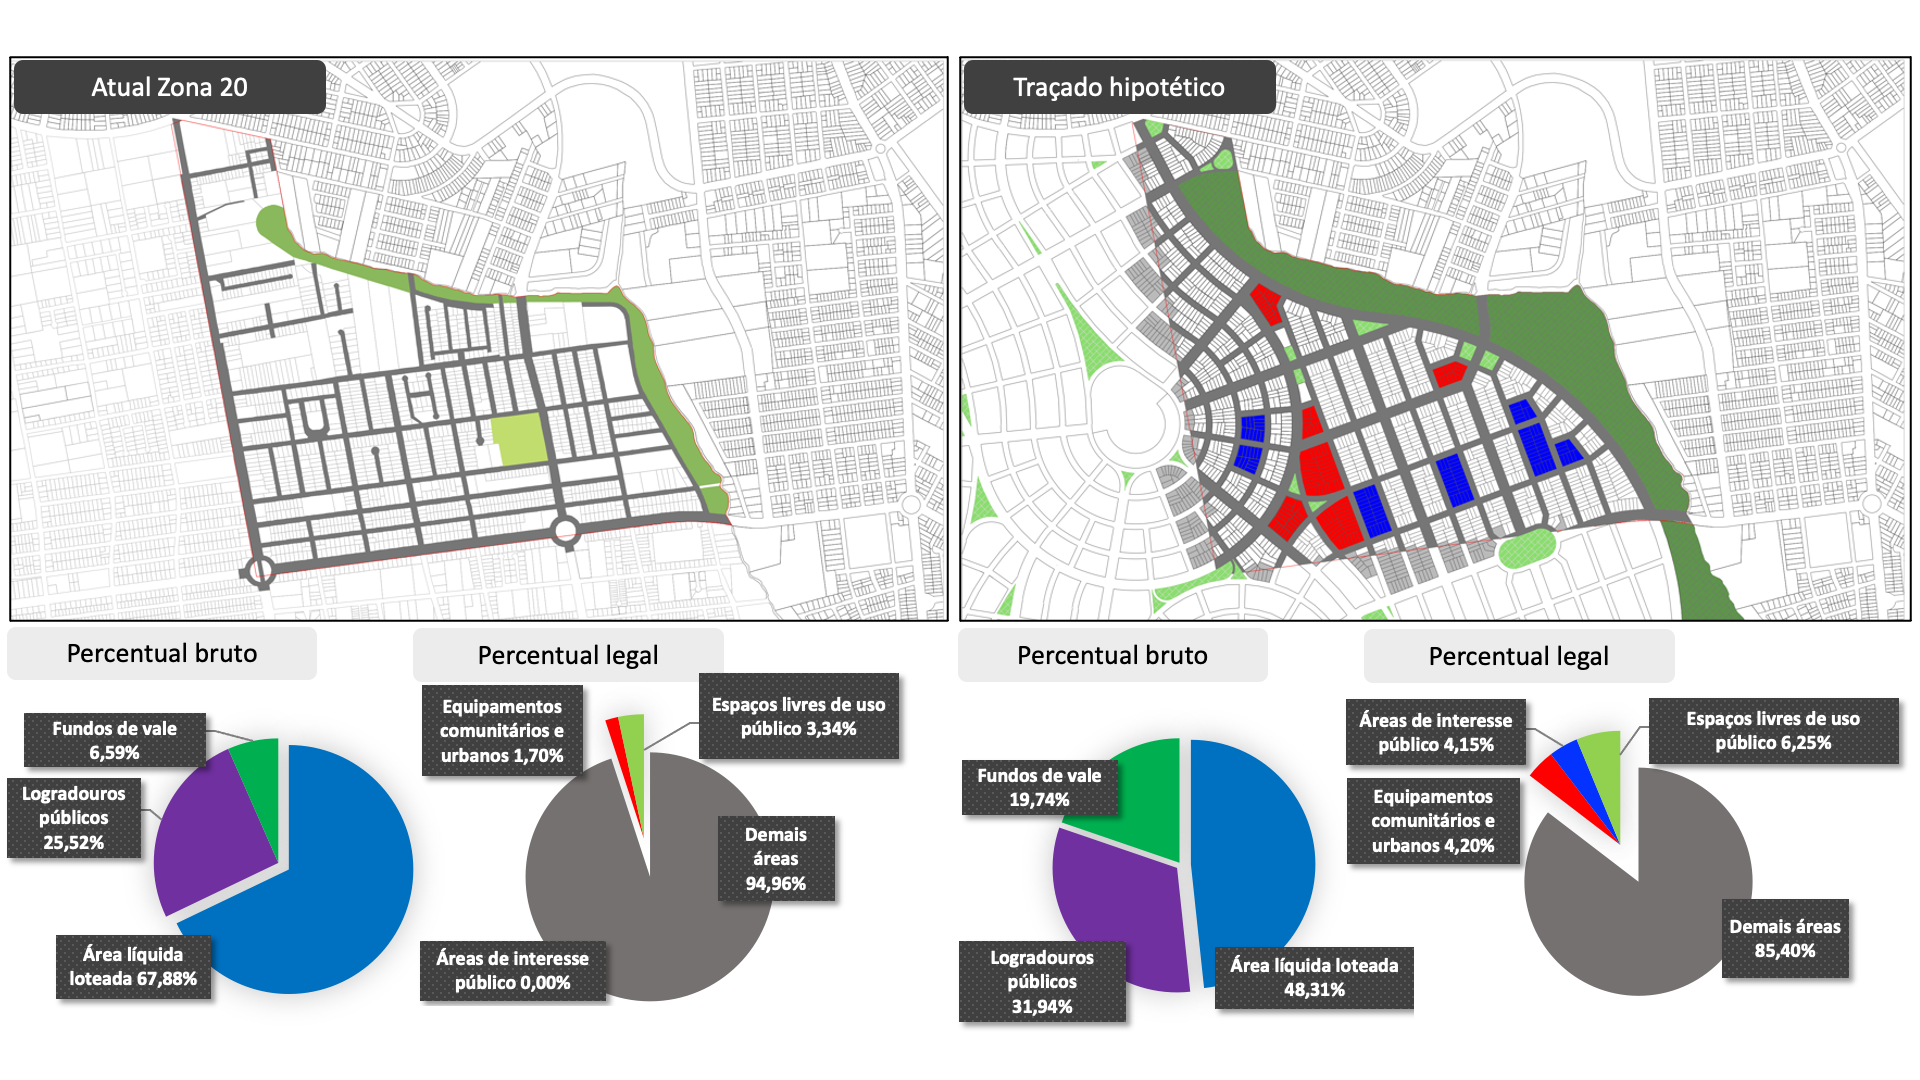
\includegraphics[width=1\textwidth]{/Users/Pancratii/GitHub/phd/Sections/Projeto_de_Pesquisa_2023-03-18_Teste/Pictures/comparativo_tracados.png}
            \captionsetup{labelfont=bf}
            \caption{Comparativo entre o traçado existente (à esquerda) e o traçado hipotético projetado (à direita). \textbf{Fonte:} Costa, 2020 (adaptado).}
            \label{fig:comparativo_tracados}
        \end{figure} 

        \begin{center}
        . . . . .
        \end{center}

        A principal evidência que me trouxe até aqui foi a existência de traçados urbanos adequados à topografia do sítio e de traçados feitos à revelia do relevo – estes últimos relacionados a diversos problemas, sendo oriundos daquilo que chamo '\textit{modus faciendi} atual' (Costa \textit{et al.,} 2020). Pude perceber isso em diversas cidades, e não foi diferente com Maringá-PR, meu local de estudo e experimentação até o momento. Nela, o traçado do plano original da cidade – projetado por Jorge de Macedo Vieira – se encaixa na primeira categoria, e o traçado das expansões urbanas – desenvolvido sobre o parcelamento rural da Companhia – na última.  

        O primeiro grupo congrega traçados urbanos orgânicos, com elementos interdependentes que, em geral, não são serializáveis ou intercambiáveis. Tais traçados podem ser oriundos tanto de um desenvolvimento espontâneo como de um processo de planejamento. E, em ambos os casos, o que se vê é um processo de formação ou desenvolvimento projetual mais complexo e elaborado, e, consequentemente, mais prolongado no tempo, adequando-se de modo particular às características físicas do sítio. 

        Já o segundo grupo congrega traçados não-orgânicos e intercambiáveis, oriundos do \textit{modus faciendi} atual. Neles, é possível observar uma lógica `mecanicista' subjacente, na qual prioriza-se um retorno financeiro ligado à venda de lotes, dispostos geralmente em quadras ortogonais.

        O resultado da aplicação indiscriminada de traçados abstratos, de concepção alheia ao contexto no \textit{modus faciendi} atual são ``territórios descontínuos e paisagens contraditórias'' (Strappa, 2018, p. 11, tradução nossa). Loteamentos e loteamentos que `brotam' como fungos a partir das cidades, de suas franjas e conexões.
            \footnote[4]{A expressão `fungos' foi utilizada pelo professor Philippe Daverio (2018), no contexto das cidades italianas, cuja expansão se dá de modo diferente ao que ocorre no Brasil (cf. Indovina, 2009). No entanto, tanto lá como em ultramar, muitas vezes ocorre o surgimento de empreendimentos urbanos (\textit{i.e.,} loteamentos) em locais inusitados, conectados às áreas urbanas consolidadas apenas por meio de uma pequena estrada, assim como os fungos também se reproduzem e espalham `em rede'. Portanto, a analogia permanece válida.} 
        Geram-se, assim, manchas urbanas formadas por traçados desconexos entre si. E o que se percebe é uma tendência à segregação dessas novas áreas urbanas, bem como uma diminuição da mobilidade, com a sobrecarga das poucas vias de acesso – em geral íngremes.

        Além disso, não há uma distinção clara ou uma integração sustentável entre a mancha urbana e o território natural e produtivo. Diversas ruas fazem `incursões' em áreas que, por sua morfologia e características naturais, deveriam ser preservadas. E, desse modo, o que ocorre não é uma integração entre a cidade e o campo, ou o dissolver das estruturas urbanas no território circunstante, mas sim uma espécie de `corrupção' de todos: cidade, campo e natureza.

        \begin{center}
        . . . . . 
        \end{center}

        É verdade que, sobretudo na primeira metade do século XX, houve ideários a tentar sanar essa situação, focando sobretudo na cidade enquanto habitat humano que deveria ser melhorado: estética, logística e funcionalmente. E isso por meio da relação da cidade-campo, da densidade, de determinados arranjos formais do traçado ou da dissolução da cidade tradicional em favor de utopias. Enquanto isso, nos últimos 50 anos, viu-se um emergir de considerações ambientais, não mais da cidade, mas da `paisagem'.
            \footnote[5]{As definições de `paisagem', \textit{`landscape'} e \textit{`paesaggio'} serão destrinchadas no momento oportuno.} 
        E, mais recentemente, podemos ver a ideia de \textit{`landscape'} enquanto \textit{`framework'} das cidades e regiões dentro do chamado \textit{`landscape urbanism'} (Waldheim, 2016). No entanto, em nenhum desses casos é possível identificar um estudo metódico do processo de morfogênese, sobretudo dos assentamentos espontâneos. Isso só se fez visível no arcabouço teórico-metodológico da escola italiana de tipomorfologia urbana – pouco conhecida e divulgada, precisamente por ser uma 'escola' e não um 'ideário' com princípios a aplicar por toda parte. E, ainda assim, a escola italiana trata de leitura e análise urbano-territorial, no entanto sua ênfase projetual se dá na escala das edificações, ou em projetos urbanos (\textit{`masterplan'}). Ou seja, ou oito, ou oitenta.

        Desse modo, não existem diretrizes claras para projetar traçados de maneira coerente e orgânica, sobretudo conforme o conceito de \textit{rendimento} urbano. Ademais, mesmo nos casos dos quais é possível extrair alguma diretriz, percebe-se, como sobredito, que tais casos não são feitos do mesmo modo que os traçados urbanos costumeiramente são feitos – ao menos no Brasil –, \textit{i. e.,} por loteamentos (bidimensionais) – e não à maneira de \textit{masterplan}, em que os edifícios (tridimensionais) – ou ao menos seus volumes – são projetados \textit{a priori} (Maretto, 2018; Maretto, Costa e Rego, 2023); afinal, estou falando de `traçado' (\textit{urban shape}) e não de `forma' (\textit{urban form}). E é diante desse problema que me pergunto: `como projetar um traçado urbano morfologicamente adequado ao contexto?' 

        O que pretendo, portanto, é desenvolver um conjunto de diretrizes para o projeto de traçados urbanos. Traçados esses que devem ser morfologicamente adequados. Diretrizes essas que possam ser aplicadas em diferentes contextos. E meu intuito com isso é gerar uma alternativa ao \textit{modus faciendi} atual. Para isso, eu preciso ampliar o horizonte do conceito de \textit{rendimento} para além do traçado urbano enquanto algo estanque, tornando-o aplicável na dinâmica da realidade. Ou seja, devo relacionar o conceito de \textit{rendimento} urbano com o processo de expansão urbana e com as estruturas naturais e antrópicas que lhe servem de \textit{framework} – nesse caso, expansões extra-urbanas, peri-urbanas e/ou intra-urbanas.
            \footnote[6]{Eu falaria aqui, também, de reestruturação urbana – no sentido caniggiano do termo. No entanto, penso que estabelecer um modo de fazer cidades e territórios adequado ao contexto servirá tanto para `expansões' quanto para `reestruturações' urbanas.} 
        E, a partir disso, desenvolver um artefato (conjunto de diretrizes) que possa ser utilizado por todos aqueles que projetam traçados, e, com isso, produzem cidades e territórios, tais como projetistas, empreendedores, imobiliaristas, legisladores, gestores, pesquisadores, docentes, alunos. Destarte, se falar em mudança de paradigma é de uma presunção deveras arrogante, faz-se mister, porém, falar em `alternativa' ao modo de fazer traçados urbanos hoje em voga.

        \begin{center}
        . . . . .
        \end{center}

        Uma justificativa razoável para a presente empresa é a ausência de estudos prescritivos para traçados urbanos sob a luz do \textit{rendimento} urbano e de sua prerrogativa de coerência entre traçado e contexto. No campo da morfologia urbana, existem estudos de observação e análise de traçados urbanos, como a metodologia \textit{Morpho} (Oliveira e Silva, 2013; Oliveira e Medeiros, 2016), mas que não consideram a topografia; ou estudos que consideram as formas do terreno no território e outros fatores ligados à sustentabilidade ambiental (Fanta \textit{et al.,} 2022), mas que não adentram no tocante específico dos traçados urbanos e de seus formatos. Ambos de caráter não-prescritivo. Neles, vê-se a ausência de diretrizes prescritivas para o desenho das cidades, sobretudo diretrizes que agreguem \textit{savoir-faire} de diferentes áreas do conhecimento. Até existem manuais, porém, ou eles datam de mais de um século, como é o caso de Unwin (1909) e Sitte (1889), ou, mais recentemente, tratam mais de aspectos relacionados ao `aproveitamento' e infraestruturas de loteamentos, como é o caso de Mascaró (2003); e, em ambas as situações, pouco ou nada se fala do aspecto ambiental do traçado urbano. Mais recentemente, até surgem novos manuais, porém, mais voltados ao desenho urbano na escala da rua do que na escala do traçado: canteiros, mobiliário, distribuição das faixas e arborização são seus objetos, não a morfologia urbana em escala mais ampla. Há diretrizes, e até métodos para a análise que dá suporte a um possível processo de projeto, mas não uma prescrição endereçada diretamente a tal. Há ainda o método de projeto desenvolvido no âmbito dos workshops W.A.M. (Maretto, 2018), e aquele presente no trabalho de Saverio Muratori para o programa habitacional INA-Casa (Maretto, Costa e Rego, 2023) – ambos prescritivos. Porém, em ambos, ainda que havendo alguma consideração pela topografia (sobretudo no exemplo muratoriano), parte-se de uma realidade edificada pré-existente, com tecidos urbanos históricos, ou em áreas novas (ou de intervenção) nas bordas de uma realidade construída já consolidada. E isso sem falar que aqui tratamos de projetos \textit{à la masterplan}, ou seja, de um processo que depende do arquiteto e de um ente que possa levar a cabo toda a empreitada, diferente do processo de formação da cidade, com seus diferentes atores e fontes de receita (Alexander \textit{et al.,} 2013).

        Ou seja, não há diretrizes atuais para o projeto de traçados urbanos partindo da característica mais crua e rudimentar de uma cidade, daquilo que lhe é subjacente, a saber: a forma de sua estruturação natural. Esta, com toda sua complexidade, reflexo de relações orgânicas de interdependência entre orografia e hidrografia – moldadas pelo clima, regime pluviométrico, e tipos de solo – recebe todos os impactos do processo de urbanização. Mais um fator a ser observado em um conjunto de diretrizes – o da sustentabilidade ambiental, vinculada ao formato dos traçados, com a qualidade inerente à sua morfologia. Adaptação dos formatos do traçado urbano, que são subjacentes às formas edificadas e que conferem qualidade ao ambiente construído, disposto sobre um relevo natural. Estes são os pontos fulcrais que justificam um estudo como a tese aqui proposta, pois, por meio de um conjunto prescritivo de diretrizes que visa incrementar um processo já existente de projetação de traçados urbanos, explicita-se ser possível associar \textit{rendimento} urbano e `rendimento’ econômico, mostrando que os diversos interesses dos diferentes atores que atuam na cidade podem convergir para um bem comum, no qual todos saiam ganhando.

        Ademais, se é verdade que consegui projetar um traçado urbano adequado a um determinado contexto, não necessariamente é verdade que uma outra pessoa o conseguirá fazer em outro contexto. Faz-se mister pôr à prova o estratagema que utilizei. E como tornar isso palpável? Por meio de um software ou algoritmo, no qual fosse necessario fornecer apenas algumas instruções, dar um \textit{input}? Bom, nesse caso eu precisaria de uma equipe, e diretrizes já delineadas e organizadas metodicamente, coisa que é inviável no prazo de quatro anos de um doutorado – ao menos para um leigo em linguagem de programação. Então por meio de um método, com um passo-a-passo? Não necessariamente, posto que isso engessaria a aplicação do projeto quando em diferentes contextos e circunstâncias. Bem, nesse caso, por exclusão, cheguei à determinação de que são necessárias diretrizes de projeto, um conjunto de diretrizes para o processo de projetar traçados urbanos morfologicamente adequados ao contexto. 

        %Método
        Para desenvolver tais diretrizes, lanço mão da \textit{Design Science Research} (DSR) como método de pesquisa (Dresch \textit{et al.,} 2013; Lacerda \textit{et al.,} 2015), por ser um método prescritivo que visa a melhoria de processos já existentes. No caso em questão, prescritivas são as diretrizes de projeto, e a realidade ou processo existente a ser melhorado é o processo de projeto de traçados urbanos.

        Fulcrais na DSR são: o desenvolvimento de um `artefato' (aqui, o conjunto de diretrizes), e a avaliação e comunicação dos resultados por e para os \textit{stakeholders} (que, no caso em questão, são profissionais, gestores, pesquisadores, docentes e estudantes que lidam com o processo de projeto de traçados urbanos). Tal método de pesquisa é constituído por fases, sendo elas: (1) consciência do problema; (2) sugestão; (3) desenvolvimento; (4) avaliação; e (5) conclusão. Tais fases se retroalimentam entre si, e seus produtos são: (a) proposta; (b) esboço; (c) artefato; (d) mensuração; e (e) resultados (Vaishnavi e Kuechler, 2021 [2004]).

        %[17NOV2023 19:56 UEM] 
        Na primeira etapa desse método, deve-se ``identificar e compreender o problema que [se] deseja estudar e solucionar'', bem como ``definir qual é a \textit{performance} necessária para o sistema em estudo'' – performance essa que será medida posteriormente (nas etapas de desenvolvimento e avaliação) com parâmetros extraídos da revisão de literatura e de um estudo de caso. Na segunda etapa, são sugeridas possíveis soluções para o problema de maneira abdutiva – nesse caso, por meio da definição de três situações para traçados hipotéticos. Na terceira etapa, ocorre o desenvolvimento de um dos artefatos propostos na segunda etapa – ou seja, um conjunto de diretrizes que serão extraídas a partir do projeto desses traçados hipotéticos. As diretrizes que se mostrarem adequadas na solução do problema (relativo ao processo de projeto de traçados morfologicamente adequados) serão avaliadas em uma quarta etapa (Dresch \textit{et al.}, 2015, p. 79; Vaishnavi e Kuechler, 2021, pp. 11-13). E é essa disposição das etapas que se desdobra na formatação dos capítulos desta tese.

        Na presente pesquisa, associo a DSR com estratégias como estudo de caso, modelagem, simulação e grupos focais, de modo a compreender a realidade na qual pretendo intervir, identificar diferentes possibilidades dentro da realidade em questão, desenvolver um arcabouço de soluções, e verificar se tais soluções são aplicáveis em outras realidades.

        Assim, para preencher tal lacuna e alcançar o objetivo acima proposto, na senda da \textit{Design Science Research}, fazem-se necessárias as seguintes etapas, que se refletem no delineamento da pesquisa: 
            \begin{itemize}
                \item revisar conceitos e métodos tanto atinentes ao processo de projeto de traçados urbanos como à morfologia urbana, particulamente àqueles afins ao conceito de \textit{rendimento}; 
                \item buscar soluções semelhantes que já tenham sido aplicadas (como \textit{guidelines, patterns,} métodos, leis, manuais, livros) na classe de problema em questão (\textit{i.e.,} ausência de método de projeto), além de selecionar e esboçar um tipo de solução a ser desenvolvida;
                \item efetuar um estudo de caso sobre Maringá, com levantamento documental e cartográfico, leitura morfológica e revisão de literatura acerca do projeto original, das expansões urbanas, do parcelamento rural e das diretrizes viárias, bem como revisão da legislação atual; %e entrevistas com \textit{stakeholders} para entender as premissas, motivações e o processo de projeto no \textit{modus faciendi} atual; 
                \item estabelecer um protocolo para o desenvolvimento do conjunto de diretrizes; 
                \item desenvolver um conjunto de diretrizes piloto por meio de modelagem e simulação (com traçados urbanos hipotéticos); 
                \item avaliar um conjunto de diretrizes por meio de comparativo com legislação, situação, morfologia e \textit{modus faciendi} atuais (para aferir viabilidade), e por meio de grupos focais (para avaliar aplicabilidade em outros contextos); e, por fim, 
                \item refinar e sintetizar as diretrizes do conjunto.
            \end{itemize}

        \begin{center}
        . . . . .
        \end{center}

            \section*{Estrutura da Tese}

            A presente tese, destarte, é estruturada em três 'partes': a primeira, 'consciência'; a segunda, 'desenvolvimento'; e a terceira, 'avaliação'. Na primeira parte, estão presentes o estado da arte, a análise do contexto em que a tese será aplicada – qual circunstância será melhorada/refinada – e a definição de novos termos e conceitos pertinentes à tese aqui desenvolvida. Na segunda, as diretrizes de projeto são extraídas de projetos piloto de traçados urbanos seguindo um protocolo. E, por sua vez, a terceira parte é uma avaliação das diretrizes de projeto por parte dos \textit{stakeholders} do processo de projeto de traçados urbanos, \textit{i.e.,} profissionais, gestores, docentes e estudantes – ou seja, nessa última parte as diretrizes são testadas por terceiros alheios à feitura desta tese, de modo a avaliar se tais diretrizes (artefato) são realmente aplicáveis à realidade, ao meio para o qual foram desenvolvidas, a saber, escritórios (públicos ou privados), ateliês de projeto e salas de aula; e, em seguida, são sistematizadas.

            A primeira parte é dividida nos seguintes capítulos:
            \begin{enumerate}
                \item O traçado da cidade: no primeiro capítulo é feita a revisão assistemática de literatura
                
                \item Maringá, um novo estudo de caso: no segundo capítulo é feito um estudo de caso sobre Maringá, com levantamento documental e cartográfico, leitura morfológica e revisão de literatura acerca do projeto original, das expansões urbanas, do parcelamento rural e das diretrizes viárias, bem como revisão da legislação atual.
                
                \item A escolha de uma solução: revisão sistemática de literatura para identificar 
            \end{enumerate}

            Na segunda parte, encontra-se o capítulo intitulado `o projeto de traçados hipotéticos'
                Parâmetros: quantitativos (número de lotes, área verde por habitante, área loteável, área pública), leis, etc.
                O projeto de traçados hipotéticos: aqui, apresento três pilotos, projetos hipotéticos de traçados urbanos. O primeiro foi desenvolvido durante o mestrado, sozinho, sobre um promontório inteiro, ou seja, uma espécie de \textit{tabula rasa} e um piloto inicial de traçado urbano. O segundo traçado foi desenvolvido durante enquanto orientei um projeto de iniciação científica, considerando algumas pré-existências antrópicas da área estudada, como diretrizes viárias, avenidas e faixas de domínio pré-existentes; portanto, um piloto de desenvolvimento semi-autônomo das diretrizes por parte de \textit{stakeholders} (eu e o aluno orientado), ao mesmo tempo que abarcando áreas intra-urbanas, o que indica a possibilidade de uso das diretrizes em áreas urbanas sub-utilizadas, ou na pesquisa e no estudo comparativo (acadêmico) de possíveis alternativas ao modo como atualmente se projetam traçados urbanos. E o terceiro foi desenvolvido no âmbito desta tese, considerando um processo de expansão urbana cujos módulos são os lotes rurais paulatinamente ocupados por loteamentos estruturados por uma estrutura comum (eventualmente um \textit{framework}). Neste capítulo, assim, são apresentados tais traçados e o passo-a-passo de seu desenvolvimento projetual, o que nos leva ao capítulo seguinte.
                Diretrizes projetuais: Neste capítulo, as diretrizes projetuais extraídas do desenvolvimento projetual dos pilotos são sistematizadas dentro de um esquema que permite diferentes alternativas, de modo a proporcionar diversas soluções projetuais em diferentes contextos, porém, sempre mantendo a mesma qualidade de morfoadequação do traçado ao contexto.
                Comparativo com existente: (número de lotes, área verde por habitante, área loteável, área pública), leis, etc.
                
            Já na terceira parte, encontram-se os seguintes capítulos:
            \begin{itemize}
                \item Grupos focais e \textit{feedback}
                \item Diretrizes projetuais
            \end{itemize}


    
    \part[Consciência]{Consciência}

        \chapter[O traçado da cidade]{Revisão de literatura}

        Precisamos pensar a rua, o bairro, a cidade como conjuntos. Cada um deles deve colaborar com o todo. A ideia não é minha, mas de Sir Raymond Unwin (1909, p. 288). 
            \footnote[10]{``We need to think of the street, the district, the town as larger wholes, and find a glorious function and a worthy guidance for the decorative treatment of each plot and each house in so designing them that they shall contribute to some total effect. \textit{For is it not a finer thing to be a part of a great whole than to be merely a showy unit among a multitude of other units?}'' (Unwin, 1909, p. 288, destaques nossos).}
        Esse princípio – da subordinação das partes ao todo – é o mesmo que rege o \textit{``rendimento''} em sua concepção original, de que tratei em minha dissertação de mestrado (Costa, 2020). Um traçado morfologicamente adequado, assim como proposto nesta tese, é um traçado com \textit{``rendimento''}. E, partindo desse ponto, ressoa a questão de pesquisa: `como projetar um traçado urbano morfologicamente adequado?'

        Bem, vamos por partes: falemos primeiro sobre o ato de projetar, ou, mais especificamente projetar traçados urbanos, para, em seguida, falarmos de adequação morfológica. Mas, antes de mais, é necessário refrescar a memória acerca do que é \textit{``rendimento''.} No âmbito da escola italiana de tipomorfologia, \textit{``rendimento''} é ``a dialética entre uma ação antrópica e uma reação ambiental, constituída pelo menor ou maior esforço com que o ambiente tenderá a reabsorver o resultado daquela ação'' (Caniggia e Maffei, 2008, p. 52, tradução nossa). Ação que é basicamente a intervenção feita por um indivíduo ou grupo durante um intervalo de tempo. Ambiente que é um conjunto unitário, resultante de diversas intervenções feitas ao longo do tempo, como um amálgama. E reação que é basicamente `o que ocorre depois que a ação é feita', um desencadear de novas ações que modifica o ambiente a partir dessa ação `inicial'. Quanto maior o \textit{rendimento} de uma intervenção, menor o esforço do ambiente para absorvêla e ``torna-la coerente com seu contexto'' (Rebecchini, 2008, p. 107, tradução nossa). Desse modo, o \textit{rendimento} diz respeito a uma relação de equilíbrio entre cada ação (parte) com o ambiente (o todo), sendo a dialética entre algo novo e um universo já existente. Ou seja, em princípio, o \textit{rendimento} pode ser entendido como ``grau de coerência com o contexto'' (Maffei, 2003, p. 82, tradução nossa).

        Em minha dissertação de mestrado, ainda, desenvolvi uma nova acepção do conceito de \textit{rendimento}, intitulada ``rendimento urbano''. Isso porque até então o conceito de \textit{rendimento} era aplicado apenas na escala da edificação – \textit{rendimento} edilício (Caniggia e Maffei, 2008; Caniggia, 1963; Cataldi, 2015; De Martin, 2009; Rebecchini, 2008; Dalla Negra, 2015; Marzot, 2015) – e na escala do território – \textit{rendimento} territorial (Carlotti, 2015). Não havia ainda a aplicação desse conceito na escala da cidade, tanto menos em língua portuguesa. E o resultado da pesquisa redundou no ``rendimento urbano'' ser concebido como ``a coerência intrínseca entre o traçado da forma urbana e o contexto natural'' (Costa, 2020, p. 52).

        Ora, se o \textit{rendimento} é uma dialética entre algo novo e algo já existente, podemos estabelecer como exemplo um traçado urbano como sendo esse `algo novo' e um território como `algo já existente'. E, dito isso, é hora de retomarmos o fio da meada. Falemos de projeto de traçados urbanos agora, para falarmos de adequação morfológica e território depois.

        Para entender o traçado da cidade e o que fazer com ele, proponho duas revisões de literatura. A primeira é uma revisão assistemática, com os principais autores relacionados ao projeto de traçados urbanos, de modo a verificar que parâmetros são divisados por esses autores como qualidades e parâmetros balizadores de projeto. Além disso, tal revisão serve para identificar em que medida obras consagradas – no Brasil e no exterior – ao longo do tempo se aproximam ou não do conceito de \textit{rendimento} e da noção de organicidade a ele associada. Bem como da relação entre cidade e território (sobre o qual se expande).

        A segunda é uma revisão sistemática de literatura para identificar manuais e \textit{guidelines} contendo diretrizes de projeto, no Brasil e no exterior, com o intuito de verificar quais desses manuais e \textit{guidelines} empregam parâmetros de projeto que possam ser relacionados ao conceito de \textit{rendimento} e às qualidades identificadas na revisão assistemática de literatura. Desse modo, será possível identificar artefatos semelhantes ao desenvolvido aqui.

        Os autores utilizados na revisão assistemática de literatura são: Raymond Unwin (1909), Camillo Sitte (1992), Vicente del Rio (1999), Juan Luís Mascaró (2003), Matthew Carmona \textit{et al.} (2003), Matthew Carmona e Louie Sieh (2004), Matthew Carmona e Tiesdell Steven (2007), Frederick Steiner e Kent Butler (2007), Gianfranco Caniggia e Gian Luigi Maffei (2008), Álvaro Rodriguez (2010), Spiro Kostof (2014), Gerd Wilhelm Kohlhepp (2015), Vitor Oliveira (2016, 2018), Charles Waldheim (2016), Gareth Doherty e Charles Waldheim (2016), Huimin Ji e Wowo Ding (2021), e Václav Fanta \textit{et al.} (2022).

            %\begin{itemize} %Livros para leitura (ver quais parâmetros que eles dão como qualidade e que devem ser levados em conta no momento de projetar um traçado urbano)
              %  \item Unwin
                %\item Sitte
                %\item Mascaró %(para tratar do modus faciendi atual, de como se ensina ou o que se consulta na hora de projetar traçados)
                %\item Del Rio
                %\item Kostof
                %\item Vitor Oliveira
                %\item Caniggia e Maffei
                %\item Álvaro Rodriguez
                %\item Waldheim (os dois livros)
                %\item Kohlhepp
                %\item Fanta et al.
                %\item Legislação (brasileira e local) %Levar em conta que isso pode variar no caso de outros países
                %\item Carmona
                %\item Manual de urbanismo (Gislaine)
            %\end{itemize}
                
        Unwin (1909) por conta da vinculação de Jorge de Macedo Vieira com a sua prática projetual, e por ser um dos clássicos da literatura de projeto, mas que, diferente de outros autores, não foi traduzido para o português. Sitte (1992) porque Unwin é tributário de Camillo Sitte. Mascaró (2003) e Del Rio (1999) para entender o que é levado em conta no Brasil no momento de projetar traçados, sendo utilizado nos currículos das universidades brasileiras. Wo e Ding (2021) para definir o conceito de traçado urbano empregado nesta tese. Vitor Oliveira (2016, 2018) por suas recentes descobertas no campo da morfologia urbana e sua aplicação no projeto de traçados urbanos. Caniggia e Maffei (2008) por trazerem à baila o modo como as cidades se estruturam organicamente. Álvaro Rodriguez (2010) e Charles Waldheim (2016) por conta da evolução do processo de urbanização e da atual relação entre o território e a cidade – e, por consequência, seu traçado. Em seguida, Kohlhepp (2015) e Fanta \textit{et al.} (2022), para entender o tipo de parcelamento rural do território de Maringá, sobre o qual novos traçados urbanos vêm sendo projetados. E, por fim, a legislação, de modo a ter um panorama daquilo que pode ser aplicado na prática no local utilizado para estudo.
   

        \begin{center}
        . . . . .
        \end{center} 

            %Mascaró, p. 13
            ``Todo sítio tem na topografia suas caracteristicas principais.'' A frase não é minha, mas de Juan Luis Mascaró (2003, p. 13), autor de um dos mais conhecidos manuais de ``Loteamentos Urbanos''.

            \begin{quotation} 
                \textit{Obviamente, nas declividades, na uniformidade, no tamanho dos morros e das bacias e em outros aspectos do relevo estarão os mais fortes condicionantes do traçado urbano.
                Igualmente, cada sitio tem seu ecossistema natural que, em maior ou menor grau, e alterado e agredido quando sobre ele se faz um assentamento urbano. O novo sistema ecologico criado podera ser agradavel ou não, estável ou instável, econômico ou antieconômico, dependendo, em grande parte, do critério com que o urbanista o trata.
                Não se pode dar uma regra geral, mas geralmente os sistemas mais agradáveis são aqueles que contém menores alterações, tornando-se mais econômicos e estáveis no tempo.
                Com os modernos equipamentos de grande capacidade para os movimentos de terra que tanto orguIham os técnicos dessa area tem-se condições técnicas de criar sítios com topografia totalmente artificial. Frequentemente se vê áreas de relevo complexo serem aterradas e desbastadas completamente, para ali ser criado um perfil topográfico mais simples, objetivando facilitar a subdivisão e a posterior edificação das residencias. Mais simples, sim; melhores, não. 
                Os assentamentos humanos que geralmente mais agradam são aqueles que parecem ter se desenvolvido de forma espontânea, aqueles lugarejos que aparecem como encravados na propria natureza. Curiosamente, esse tipo de assentamento que respeita a natureza é mais economico para implantar, porque dispensa os grandes movimentos de terra. Também se torna mais econômico de manter, porque é ecologicamente mais estável. 
                [E] Visto dessa outra perspectiva, evidencia-se que o desenho urbano não pode ser feito resolvendo apenas o problema na planta. Para se obter um bom desenho, deve-se trabalhar em suas três dimensões, levando em consideração que as soluções escolhidas necessitam se adaptar e serem oriundas das condições topográficas. 
                Embora isso seja muito claro, é frequente encontrar nos compêndios de desenho urbano diferentes traçados alternativos, colocados como se fossem de livre escolha, como se nada tivessem a ver com a topografia.}
            \end{quotation}

        \begin{center}
            . . . . .
        \end{center} 

\section{Unwin}
        
        Raymond Unwin, em seu tratado ``Town Planning in Practice: an introduction to the art of designing cities and suburbs'' (1909), expõe em detalhe diversos casos, os quais analisa e dos quais toma exemplo para diretrizes de projeto. Algumas dessas diretrizes surpreendentemente à frente de seu tempo e que permanecem ainda hoje por implementar, como veremos adiante. 

        Unwin divide sua obra em 12 capítulos, tratando sobre \textit{``Town planning''} e \textit{``Site planning''}, em duas escalas distintas, ainda que, segundo o autor, sem uma linha de demarcação. No \textit{``town planning''}, ``a primeira consideração deve ser a conveniência geral da cidade e o arranjo das principais vias''. Enquanto isso, no \textit{``site planning''}, a consideração recai no ``arranjo das edificações e no desenvolvimento do local" (Unwin, 1909, p. 289, tradução nossa). 
            \footnote[11]{``Between site planning and town planning there is no line of demarcation, and the main principles which govern the one would also apply to the other; but there is none the less a considerable difference between the two, and it is convenient to treat them separately, because in site planning the first consideration will be the arrangement of the buildings and the development of the site to the best advantage, whereas in town planning the first consideration must be the general convenience of the town, and the arrangement of the main roads. When the main roads have been laid down and the main traffic requirements have been provided for, the spaces left between these through roads can be developed more from the point of view of making the best of the sites for the buildings, and less from the point of view of public convenience.'' (Unwin, 1909, p. 289).} 
        Desse modo, minha atenção recai sobre o \textit{``town planning''}.

        O manual de projeto de Unwin se inicia afirmando que é necessário classificar as cidades com diferentes tipos de traçado: aqueles ``que evoluíram por meio do crescimento natural'' e aquelas cidades ``que foram projetadas em diferentes períodos'' (Unwin, 1909, p. 16, tradução nossa). E, enquanto no mundo clássico, muito se vê de ângulos retos indo de Norte a Sul (pp. 45-46), nas cidades medievais as irregularidades parecem ter um planejamento, diferente do que estamos acostumados a pensar. Um planejamento feito no nível do transeunte, no olho (p. 52).\footnote[12]{``[The] setting out of the buildings was done largely on the ground by the eye, \textit{and not transfered from a paper plan}.'' (Unwin, 1909, p. 52, destaques nossos).}
        \footnote[13]{Essa observação é importante, pois perpassará toda a obra de Unwin.}

        Em um passado mais recente, durante a Renascença, nos séculos XVI e XVII, o renascimento das artes e estudos clássicos teve um papel decisivo no planejamento das cidades, pois ``a Renascença trouxe consigo o poder e a coragem para lidar com o planejamento em larga escala e desenvolveu o que se pode chamar de uma grande abordagem em esquemas de organização'' (Unwin, 1909, p. 69, tradução nossa).\footnote[14]{``[The] Renaissance brought with it the power and courage to handle town planning on a large scale, and developed what one may call a grand manner in schemes of laying out.'' (Unwin, 1909, p. 69).} E, nesse ínterim, a fundação de novas cidades tornou-se a ocupação favorita de diversos príncipes, desenhando-as com as linhas retas e formais típicas da Renascença.\footnote[15]{``[After] the troubles of the Thirty Years' War were over, the foundation of new towns and town districts in Germany became a favourite occupation of princes. (...) [These towns and discricts] are generally laid out on the straight, formal lines typical of Renaissance work.'' (Unwin, 1909, p. 69).}

        Para Unwin (p. 84), o que se desenvolveu foi uma verdadeira escola de planejadores renascentistas, cujas obras (traçados) eram desenvolvidas em grandes propriedades, com linhas rígidas e formais. E isso perdurou – ao menos na Europa – até o despontar da escola de paisagismo.\footnote[16]{``Such town planning as took place was chiefly on the land of individual owners of large estates, and was generally rigid and formal, until the influence of the landscape gardening school began to extend to the planning of streets (...) to produce curved lines, without much regard to the architectural effect of the buildings.'' (Unwin, 1909, p. 84).} O resultado disso foi que as cidades cresceram de modo caótico, com cada proprietário ``desenvolvendo sua própria terra sobre linhas que atentiam aos seus interesses ou caprichos'', resultando em traçados que deveriam prover ``o máximo número de locais para construção com o menor custo'' (Unwin, 1909, p. 88, tradução nossa).\footnote[17]{``[Towns] have been allowed to grow in a haphazard manner, each individual owner developing his own land on the lines which suited his own interest or fancy. Too often the only consideration has been to find a plan which would give \textit{the maximum number of building sites at the minimum cost.}'' (Unwin, 1909, p. 88, destaques nossos).}

        Por outro lado, porém, surgia uma outra escola de planejamento urbano, baseada nas conclusões de Camillo Sitte de que as cidades medievais eram, sim, planejadas. Não planejadas para o tráfego, mas sim de acordo com princípios artísticos (Unwin, 1909, p. 98).\footnote[18]{``Camillo Sitte, by a careful study of plans of medieval towns, came to the conclusion that these were designed on lines which not only provided completely for the convenience of traffic, but were in accordance with the artistic principles upon which the beauty of towns must depend. (...) [Now,] the Germans are (...) seeking to reproduce these, and to consciously design along the same irregular lines.'' (Unwin, 1909, p. 98).} E, para Unwin, o trabalho do planejador ``moderno'' deveria ser feito baseando-se nas mesmas linhas irregulares dos traçados medievais (p. 104).
        
        No entanto, nem só de curvas irregulares viveria o homem. Linhas mais regulares seriam úteis para o desenho da cidade, sobretudo para dar conferir um \textit{framework}, um senso de conjunto ao todo (Unwin, 1909, p. 12).\footnote[19]{``While, however, the importance of most of the principles which Camillo Sitte deduced from his study of medieval towns may be as great as the modern German school thinks, it does seem to me that they are in danger of regarding these principles as the only ones of great importance; nor do they appear to realise how far it is possible to comply with these principles in designs based upon more regular lines. Some of the irregularity in their work appears to be introduced for its own sake, and if not aimlessly, at least without adequate reason; the result being that many of their more recent plans lack any sense of framework or largeness of design at all in scale with the area dealt with.'' (Unwin, 1909, p. 112).}
        
        Desses dois modos de fazer traçados redundam duas classes de ``beleza'', uma `formal' e outra `informal'. E, a partir disso, duas classes de \textit{designers}: o trabalho dos `formais' baseado na convicção de que o tratamento deveria ser formal e regular, e o trabalho dos `informais' radicado na ideia de que a informalidade é o desejável (Unwin, 1909, p. 116). Porém, formal ou informal, cada um tem sua beleza. Um não anula o outro (p. 119).\footnote[20]{``[We] are not therefore justified in assuming either that there is any beauty in mere informality, or that informality in the work carried out by men is in any sense natural; nor, on the contrary, can we deduce from such a premise either that formality will not produce beauty or that it is in any sense unnatural for man to do his work on formal lines'' (Unwin, 1909, p. 119).}

        Unwin pontua que qualquer tentativa de copiar a natureza é fútil, posto que impossível de reproduzir. ``As formas que encontramos na natureza (...) são o resultado da mais perfeita obediência às mais complexas leis, de tal modo que poderíamos dizer que tais formas são inevitáveis'' (Unwin, 1909, p. 119, tradução nossa).\footnote[21]{``[The] forms which we find beautiful in wild nature are the result, so far as we know, of obedience the most perfect to laws the most complex, so much so that we may call the forms inevitable. (...) [W]eather and gravity, (...) materials and the chemical reactions (...) the slopes of the hills and valleys, the bend of the river, the curve of the bay, and the forms of the trees'' (Unwin, 1909, p. 119).}

        Dito isso, Unwin menciona ser importante fazer um estudo cuidadoso do sítio onde se quer intervir e de seu potencial, com atenção para as belezas naturais do lugar. É necessário lembrar que o projeto deve ser subordinado ao sítio e que qualquer formalismo deve ser visto como um meio para levar a cabo um objetivo, e não um fim em si mesmo. É necessário abranger de tudo, do formal e do informal. Não uma `terceira via', mas sim abarcar o que há de útil nos objetivos e métodos de cada (Unwin, 1909, p. 125).\footnote[22]{``The subject is, of course, a wide and difficult one; many of the words, such as `natural,' `formal,' \&c., used in discussing it have meanings difficult to define. Both schools of designers include men of such distinguished abilities and produce results of such marked beauty that we need not so much to decide between them as to seek for some third course, not exactly a \textit{via media} but perhaps a \textit{via latior} which shall embrace what is valuable in the aims and methods of each'' (Unwin, 1909, p. 125).} 
        \footnote[23]{``But the building up of a town is not accomplished by the making of such a sketch design. And even were the artist himself given absolute control of every detail of the work, he would find that modern conditions would upset many of his proportions and that the result when realised would fall far short of his mental picture. But if we plan our towns on somewhat formal lines there are effects of simple, orderly dignity which we may with some probability count on, for the conditions which we shall need to impose on the builder in order to realise them will be few and of a character fairly easily understood.'' (Unwin, 1909, p. 126).}

        Segundo Unwin, se o projetista tiver a mentalidade correta no momento de encarar o trabalho, ele deverá ``nutrir em seu coração um amor por toda a beleza natural e, ao mesmo tempo, ter sempre em mente uma apreciação clara da beleza do design específico que ele procura desenvolver'' (Unwin, 1909, p. 136, tradução nossa). Isso o ajudará a dar-se conta da importância de mesclar seu desenho ao do sítio, preservando e incorporando elementos do local em seu projeto.\footnote[24]{``If the designer is to go to work in a right spirit, he must cherish in his heart a love for all natural beauty, and at the same time have always in his mind a clear appreciation of the beauty of the definite design which he seeks to develop. (...) It will help him to realise the importance of incorporating his design with the site and of so arranging his scheme of laying out that it may serve as a means of harmonising his buildings with the surrounding country. It will save him from rashly destroying trees or other existing features which, with care, might be preserved and incorporated in his design.'' (Unwin, 1909, p. 136).}

        \begin{quotation}
            Por exemplo, um certo grau de design ordenado nas  principais linhas de um traçado urbano, sem dúvida, ajuda significativamente na compreensão e no fácil acompanhamento do mesmo, e em uma cidade planejada dessa forma, um estranho encontraria mais facilmente seu caminho, compreendendo de maneira mais simples as principais direções. No entanto, as vantagens práticas de tal arranjo ordenado do plano não exigem exatidão de simetria, a qual frequentemente não poderia ser alcançada sem um considerável sacrifício de conveniência ou beleza natural. Em tais casos, pareceria tolo pagar pesadamente para garantir um grau de simetria apenas apreciável em um plano de papel ou de cima de um balão. (Unwin, 1909, p. 137, tradução nossa).\footnote[25]{``For example, a certain degree of orderly design in the main lines of a town plan undoubtedly helps materially to the easy understanding and following of it, and in a town so planned a stranger would more readily find his way about, more easily grasp the main lines of direction. But the practical advantages of such an ordefly arrangement of the plan do not require exactitude of symmetry, which often could not be attained without considerable sacrifice of convenience or natural beauty. In such cases it would seem foolish to pay heavily for securing a degree of symmetry only appreciable on a paper plan or from the car of a balloon.'' (Unwin, 1909, p. 137).}
        \end{quotation}

        Logo, é mais importante a continuidade dos percursos do que necessariamente seu formato. É a continuidade que, efetivamente, irá contar mais na experiência do transeunte, a partir do maior ou menor número de mudanças de direção – e, em relação às curvas, as perspectivas e possíveis surpresas, assim como se vê numa cidade medieval ou outra também feita a partir do nível do pedestre, do olho humano.

        Já em locais vistos de cima, são os telhados e as linhas de telhado que mais contam (Unwin, 1909, p. 137).\footnote[26]{``On sites much overlooked from high ground, roofs and roof lines become matters of the utmost importance. In fact, the beauty or otherwise of towns, seen from a distance, depends very often rnuch more on the roofs than upon any other part of the buildings.'' (Unwin, 1909, p. 137).} E isso daqui depende não (apenas, ou não necessariamente) de um projeto paisagístico, mas sim da consideração do \textit{tipo} edificado, de códigos de postura, e, na base de tudo isso, da disposição das vias. Por exemplo, posso ter um terraceamento com telhados justapostos lado a lado que tragam à tona as formas de uma colina de maneira suave e horizontal, ou posso ter um `arranhão de gato' nessa mesma colina, com as casas dispostas uma após a outra numa fileira vertical que faz denotar ladeiras e escoamentos com declividade acentuada – que é o que mais ocorre atualmente em nossos loteamentos. De todo modo, à parte extremos de formalismo e informalismo, há espaço para divergência nas preferências de projetistas que aceitam os mesmos princípios (p. 138).\footnote[27]{``Apart from extremes of formalism and informalism, there is room for a wide divergence of individual preference among designers who accept in general the same guiding principles'' (Unwin, 1909, p. 138).}

        Para Unwin (1909, p. 140-141), a primeira obrigação de um designer é o estudo da cidade em que vai atuar, do seu sítio, da sua população e dos seus requisitos. E em sem trabalho não há como dizer que as considerações práticas vêm antes das artísticas ou o contrário, pois tais considerações são interdependentes. Desse modo, antes de qualquer projeto, é necessário realizar um levantamento de todas as condições pré-existentes.\footnote[28]{``The designer's first duty (...) must be study his town, his site, the people and their requirements.(...) In this work we cannot rightly say the practical considerations come before the artistic, or the artistic before the practical; they are interdependent. (...) Before any plan for a new town or for a scheme of town development can with prudence be commenced a survey must be made of all existing conditions'' (Unwin, 1909, pp. 140-141).}

        Mesmo ao fundar uma nova cidade, para Unwin, devem se levar em conta considerações históricas e sociológicas. Densidade da população, distribuição de áreas residenciais, comerciais e manufatureiras, distribuição de parques e espaços abertos, públicos ou não, e a extensão de cada. Além disso, devem ser levantados mapas com o desenvolvimento da cidade (Unwin, 1909, p. 141).\footnote[29]{``[E]ven in founding a new town historical and sociological considerations are by no means wanting''. (...) [D]ensity of population (...); the distribution of residential, business, and manufacturing areas (...); and the distribution of parks, public and other open spaces, and the extent of each. (...) In connection with this there should be collected a series of maps, showing as completely as possible the past development of the town'' (Unwin, 1909, p. 141)''.} Ou seja, levantamentos como os que fazemos hoje, tais como uso e ocupação, áreas livres, além da evolução morfológica da área.

        Outrossim, fotografias dos pontos descritos, mapas geológicos, e estatísticas de ventos e clima devem ser feitos. Todas a infraestrutura de tráfego deve ter sua capacidade estimada, com suas estradas, ferrovias, tramvias e hidrovias – um verdadeiro plano de mobilidade. E toda a infraestrutura de água e esgotos deve ser contabilizada (Unwin, 1909, pp. 143-145).\footnote[30]{``[P]hotographs of these taken from points of view exactly indicated on the plands would have great value (...). [G]eological maps (...) will be useful, (...) with statistics of wind and weather, from which diagrams showing the climatic conditions could be prepared. (...) All existing traffic facilities should be tabulated and their capacities estimated, whether consisting of railways', tramways, waterways, roads, subways or bridges. (...) All existing drainage systems and water supplies (...) should be scheduled.'' (Unwin, 1909, pp. 143-145).} Todas observações atuais.

        ``Quaisquer tendências marcantes de crescimento urbano devem ser observadas, com as indicações fornecidas por elas sobre as linhas mais naturais para o desenvolvimento futuro''. E, para isso, ``planos devem ser preparados mostrando com precisão as diferentes propriedades das terras'' (Unwin, 1909, p. 145).\footnote[31]{``Any marked tendencies of town growth should be noted, with the indications afforded by them as to the most natural lines for future development. (...) Plans should be prepared showing accurately the different ownerships of the land'' (Unwin, 1909, p. 145).} Basicamente observações de planejamento para o crescimento das cidades,\footnote[32]{\textit{Cf.} ``Shlomo Angel - Making Room for a Planet of Cities'', palestra veiculada pela UN-Habitat Worldwide e disponível em: https://www.youtube.com/watch?v=1GknqMC4B2o.} levantamento cadastral e \textit{land readjustment}.

        Por falar em \textit{land readjustment}, Unwin mostra sua predileção por esse método como alternativa viável à necessidade de grandes propriedades para a execução de novos traçados (como ocorreu com a dita escola renascentista e com os príncipes da Renascença). Para isso, cita o exemplo do plano de Sir Christopher Wren para a reconstrução de Londres após o Grande Incêndio. 

        \begin{quotation}
            Um ponto de grande interesse na descrição que citamos do plano de Londres de Sir Christopher Wren pode ser destacado novamente aqui, a saber, sua proposta de que os limites de todas as propriedades existentes deveriam ser ignorados. Individualmente, todos os lotes de terra deveriam ser temporariamente entregues às mãos de curadores ou comissários públicos para que pudessem ser rearranjados e a área dividida, cada pessoa recebendo de volta não exatamente o seu próprio lote, mas o mais próximo possível dele, na forma de um terreno disposto de maneira a atender às novas estradas e agrupamentos de edifícios propostos.
            (Unwin, 1909, p. 113, tradução nossa).\footnote[32]{``One point of great interest in the description which we have quoted of Sir Christopher Wren's plan of London may well be again mentioned here, namely, his proposal that the boundaries of all existing properties should be disregarded, and that the individual parcels of land should all be temporarily given into the hands of public trustees or commissioners so that they might be rearranged and the area divided, each person receiving back, not his own plot exactly, but as nearly as possible the equivalent of it in the shape of a plot of land arranged to suit the new roads and new groupings of buildings proposed. (Unwin, 1909, p. 113)''}
        \end{quotation}

        Para Unwin, ``Quando a terra é dividida em pequenos lotes, alguma forma de poder para rearranjar limites parece ser necessária para que um bom planejamento seja possível.'' No entanto, à época, havia ``muita discussão entre os urbanistas na Alemanha sobre este ponto.'' (Unwin, 1909, p. 113, tradução nossa).\footnote[33]{``Where land is held in small lots, some such power of rearranging boundaries seems necessary for good planning to be possible; but there is much discussion among town planners in Germany on this point.'' (Unwin, 1909, p. 113).} 
        
        \begin{quotation}
            Camillo Sitte e aqueles que o seguem argumentam que a necessidade surgiu principalmente devido ao tipo geométrico específico de planejamento que estava em voga antes de seu tempo, e que um tipo mais livre de planejamento, no qual maior consideração pudesse ser dada às condições existentes do local, às vias públicas e aos limites de propriedade existentes, tornaria desnecessária grande parte do rearranjo de propriedades que a escola geométrica de planejamento urbano considerava tão necessário. Argumenta-se ainda que a consideração dessas condições existentes levaria a um tipo de plano com algo do interesse e da variedade que caracterizam as cidades da Idade Média. (Unwin, 1909, p. 113, tradução nossa).\footnote[34]{``Camillo Sitte and those who follow him argue that the necessity chiefly arose owing to the particular geometrical type of planning which was in vogue previous to his day, and that a freer type of planning, in which greater consideration could be shown for the existing conditions of the site for existing roadways and property boundaries, would render needless very much of the rearrangement of properties which the geometrical school of town planning found so necessary. It is further argued that the consideration of these existing conditions would lead to a type of plan having in it something of the interest and variety which characterise the towns of the Middle Ages.'' (Unwin, 1909, p. 113)}
        \end{quotation}

        Unwin ainda enumera o levantamento de materiais construtivos e técnicas tradicionais de construção do local – o que me faz lembrar na noção caniggiana de \textit{tipo} –, o levantamento de árvores e arbustos predominantes ou adequados para o plantio – como em um plano de arborização \textit{ante litteram} –, e o levantamento de edifícios públicos, parques, espaços abertos e adequados, pontos de beleza natural, além de histórias e legendas associadas a edifícios e lugares (Unwin, 1909, p. 145).\footnote[35]{``[B]uilding materials and traditional methods of building (...), trees and shrubs prevalent or suitable for planting (...), [and] public buildings, (...) parks, (...), open spaces, (...) suitable sites[,] (...) spots of natural beauty; (...) historic or legendary associations attaching to buildings or places'' (Unwin, 1909, p. 145).} Assim, o levantamento da cidade ``deve ser preparado antes de que qualquer plano de novo desenvolvimento seja feito'', pois ``[a] cidade que busca projetar seus futuros desenvolvimentos deve primeiro se conhecer [e] (...) compreender suas próprias necessidades e capacidades'' (Unwin, 1909, p. 146, tradução nossa).\footnote[36]{``[The] City Survey (...) should be prepared before any plan of new development is made. (...)The city which seeks to design its future developments must first know itself [and] (...) understand its own needs and capacities.'' (Unwin, p. 1909, p 146).}

        O levantamento deve ser feito pelo planejador, e pode ser resultado ``do trabalho voluntário por parte dos cidadãos, e seus resultados devem constituir a base de suas instruções'' (Unwin, 1909, p. 146, tradução nossa).\footnote[37]{``[The survey] and may (...) be the result of voluntary work on the part of the citizens, and the results should form the basis of his instructions'' (Unwin, 1909, p. 146).} O planejador deve interpretar essas informações, recolhidas por meio de sua experiência e \textit{know how}, e, à luz disso, fazer seu próprio levantamento do local. ``[O planejador] considerará todas as necessidades da comunidade e todas as circunstâncias do local como constituindo, juntas, a amável mão da necessidade'' (Unwin, 1909, p. 149, tradução nossa).\footnote[38]{``[H]e will regard all the requirements of the community and all the circumstances of the site as together constituting the kindly hand of necessity'' (Unwin, 1909, p. 149).}

        \begin{quotation}
            A primeira coisa que o designer fará é garantir que tenha todos os planos necessários; estes devem incluir um levantamento de todas as árvores que valem a pena preservar no local,\footnote[39]{Preservação ambiental.} e um plano de contorno mostrando, por meio de curvas de nível, cada cinco pés de altura.\footnote[40]{5ft=1,52m.} Exceto em locais tão nivelados a ponto de serem excepcionais, esse levantamento de curvas de nível será não apenas inestimável para o designer, mas também uma fonte de economia (...) possibilitando que as estradas e esgotos sejam adaptados de forma mais precisa aos níveis do terreno. [Assim,] o primeiro dever do designer deve ser garantir a sua produção [do levantamento das curvas de nível]. Isso é essencial.\footnote[41]{Isso demonstra a importância \textit{basilar} do relevo. Digo `basilar' por estar na base. De nada (ou de não muito) adianta uma casa bonita feita em uma rua de `arranhão de gato'.} (Unwin, 1909, p. 149, tradução nossa).\footnote[42]{``The first thing the designer will do is to make sure he has all the needful plans; these should include a survey of all the trees worth preserving on the site, and a contour plan showing by the contour lines every five feet of height. Except on sites so level as to be quite exceptional, this contour survey will be found not only invaluable to the designer but also a source of economy (...) ``enabling the roads and sewers to be more accurately adapted to the levels of the ground (...) enabling the roads and sewers to be more accurately adapted to the levels of the ground. (...) [T]he designer's firts duty should be to secure its production. It is essential. (Unwin, 1909, p. 149).}
        \end{quotation}

        Após levantar essas informações, planos e sugestões, o planejador deve estudar o sítio por conta, comparando e considerando-o com as informações e sugestões coletadas, e julgando por si próprio a importância relativa de cada ponto. Ademais, também será necessário julgar quais condições e tendências são permanentes ou modificáveis no futuro. E, como o que for feito deverá permanecer ao longo do tempo, isso deverá ``ser combinado com a[s] realiza[ções] da[s] tradiç[ões] passada[s]'' (Unwin, 1909, p. 149, tradução nossa).\footnote[43]{``Having secured all the needful plans and preliminary information and suggestions, the designer will study the site for himself, comparing and considering it in connection with the information and suggestions, and judging for himself the relative importance of each point He will also have to judge how far the various conditions and tendencies brought to his notice are likely to prove permanent and how far they are likely to undergo modification in the future; for although it is the present needs for which immediate provision must be made, still in town planning, as in building, the work is of a permanent character and will remain through a long future, so that foresight must be combined with the realisation of past tradition.'' (Unwin, 1909, p. 149).} E esse julgamento virá do que ele (planejador) aprendeu como diretriz (por exemplo, com o manual do próprio Unwin). Um julgamento que deve fazer o elo entre passado e futuro.

        \begin{quotation}
            Enquanto ele percorre a área, surgirá em sua imaginação uma visão da futura comunidade, com suas necessidades e objetivos, que determinarão para ele os pontos mais importantes; e as linhas principais de seu plano devem, assim, tomar forma em sua mente antes mesmo de ele começar a colocá-las no papel.\footnote[44]{Uma descrição lúdica, mas didática, do processo de projeto de um arquiteto e urbanista.} (Unwin, 1909, p. 150, tradução nossa).\footnote[45]{ ``As he tramps along there will arise in his imagination a picture of the future community, with its needs and its aims, which will determine for him the most important points; and the main lines of his plan should thus take shape in his mind before ever he comes to put them on paper.'' (Unwin, 1909, p. 150).}
        \end{quotation}

        Desse modo, para Unwin, o planejador formará uma imagem na medida em que as necessidades da comunidade forem consideradas e atendidas. Enquanto ele estiver pensando nos principais pontos de problema, ``encontrará locais de beleza natural a serem preservados, árvores a serem protegidas da destruição, vistas distantes da cidade e visões dos edifícios imponentes" (Unwin, 1909, p. 150, tradução nossa).\footnote[46]{``The picture will grow in the designer's mind as the various needs are considered and met; and all the while he is thinking out the main points of his problem he will be finding spots of natural beauty to be preserved, trees to be guarded from destruction, distant views from the town, and views into it of the fine buildings'' (Unwin, 1909, p. 150).}

        Para Unwin, o planejador deverá tentar ``compreender a direção que as principais vias de tráfego inevitavelmente seguirão'', bem como ``quais porções de terreno serão atraentes para residências e quais oferecerão incentivos para o desenvolvimento de lojas, estabelecimentos comerciais ou indústrias'' (Unwin, 1909, pp. 149-150, tradução nossa).\footnote[47]{``[The designer will try to] ``realise the direction which the main lines of traffic will inevitably take, which portions of ground will be attractive for residences, and which will offer inducements for the development of shops, business premises, or industries.'' (Unwin, 1909, pp. 149-150).} Cada local deve ser escolhido não apenas por suas possibilidades arquitetônicas – isso também –, mas deve ser ``adequado em caráter e posição para formar centros no traçado'' de modo que a vida da cidade ou do bairro encontre um foco (Unwin, 1909, p. 150, tradução nossa).\footnote[48]{``For such purposes places must be chosen that will not only offer adequate architectural possibilities, but will also be suitable in character and position to form centre points in the plan, at which it may be reasonable to hope the common life of the city or district will find a focus.'' (Unwin, 1909, p. 150).}  

        \begin{quotation}
            Uma estação de trem existente ou provável imediatamente dará foco às linhas de tráfego e pode ser considerada um centro a partir do qual um acesso fácil deve ser fornecido para todas as partes da cidade ou distrito, uma disposição cujo caráter será afetado por todas as vias ou hidrovias existentes. Pontes existentes ou pontos onde as condições são favoráveis para a construção de pontes ou passagens subterrâneas sobre ou sob ferrovias, rios ou canais sugerirão pontos adicionais de centro no sistema de estradas, para os quais naturalmente convergiriam. O agrupamento da cidade ou subúrbio nas colinas ou encostas disponíveis também será pensado mais prontamente no local; lá, também, serão escolhidos os locais mais adequados para fábricas, onde terão todas as facilidades necessárias de transporte ferroviário e aquático, e, se possível, onde o vento predominante levará o ruído, poeira, cheiro e fumaça para longe da cidade. (Unwin, 1909, p. 150, tradução nossa).\footnote[49]{``An existing or probable railway station will at once give focus to the lines of traffic, and may be regarded as a centre from which easy access should be provided to all parts of the town or district, a provision the character of which will be affected by all existing highways or waterways. Existing bridges or points where the conditions are favourable for constructing bridges or subways over or under railways, rivers, or canals will suggest themselves as additional centre points in the system of roads, to which they would naturally converge. The grouping of the town or suburb upon the hills or slopes available will also be thought out most readily on the spot; there, too, will most easily be selected suitable sites for factories, where they will have all the necessary facilities of rail and water carriage, and, if possible, where the prevailing wind will take the noise, dust, smell, and smoke away from the town.'' (Unwin, 1909, p. 150)}
        \end{quotation}

        Depois do levantamento e da escolha desses pontos dentro do sítio, Unwin menciona a necessidade de marcar os limites e acessos das cidades e bairros. Para ele, ``é absolutamente necessário de alguma forma definir nossas áreas urbanas e, no caso de cidades grandes, delimitar e separar novas áreas e subúrbios''. E mais, é necessário ``limitar de alguma forma o tamanho das cidades''. No entanto, completa, ``até que ponto isso é possível, ainda temos que descobrir'' (Unwin, 1909, p. 154, tradução nossa).\footnote[50]{``We have no occasion, and it would therefore be a pure affectation, to seek to fortify our towns with walls, nor is it desirable that we should cause undue congestion; but \textit{it is most necessary in some way to define our town areas, and in the case ot large towns to define and separate new areas and suburbs.} It would seem desirable to \textit{limit in some way the size of towns,} but how far this may be possible we have yet to learn.'' (p. 154, destaques nossos).} 

        É necessário tirar lição das cidades do passado, mas sem necessariamente fazer uma cópia \textit{ipsis litteris} de suas soluções. Não é necessário refazer muralhas para delimitar cidades, mas sim tirar partido das áreas deixadas por elas, uma vez desfeitas. Ou aprender com o princípio de que elas seguiam o relevo. Nesse sentido, Unwin menciona que avenidas, boulevards e cinturões de parques (cinturões verdes) podem servir de exemplo (Unwin, 1909, p. 154).\footnote[51]{``Thus we may derive useful lessons from the beautiful towns of other lands and other days, not seeking to copy their features, but \textit{finding the reasons which gave rise to them and gathering some suggestions} which may in turn help to beautify our own cities. Though \textit{we shall not copy the fortified wall} of the old city, we may take from it a most pregnant suggestion of the value of defining and limiting towns, suburbs, and new areas generally. This may be done, in many ways. (...) [The] removal of inner rings has given an opportunity to replace them by wide boulevards, avenues, or belts of park land, which do to a large extent maintain the break and the definition of the old wall'' (Unwin, 1909, p. 154, destaques nossos).} \footnote[52]{Particularmente, não sou fã da ideia das avenidas do século XIX no lugar das muralhas, porém melhor avenidas do que simples `vias paisagísticas'. Penso que seja necessário mostrar esse limite, e, assim como a muralha era algo que fazia a cidade ser vista desde fora – e também desde dentro (pois você sabia que estava `dentro' da cidade) –, assim também uma avenida com um conjunto de árvores definido de maneira contínua pode fazer destacar algo identificável na paisagem. Pense em olhar ao longe a cidade de Orte, como fez Pasolini. E pense em olhar a campanha de Orvieto ou de Alviano desde dentro das muralhas da cidade. Você consegue identificar quem é um e quem é outro. Diferenciar um e outro. Cidade e campanha. Eu não consigo me render à ideia de não-cidade que é essa cidade território que transformou a campanha num grande organismo parasitado por um fungo de estruturas antrópicas – casas esparsas ligadas por estradas. Um fungo, não um organismo com células que formam tecidos, como o é uma cidade. Nesse sentido, concordo plena e totalmente com o Daverio: é necessário fazer um restauro da paisagem. Há quem diga que isso não tem retorno e não há como voltar a isso, e que a memória coletiva das pessoas talvez sequer lembre disso. Eu, porém, estou com as viúvas que choram essa perda e digo que isso tem de ser restaurado: essa paisagem bem definida entre cidade e campo (assim como o fazem na Alemanha e Inglaterra, a tal ponto das áreas industriais estarem escondidas em maciços florestais, de modo a não incomodar e ferir o olhar dos cidadãos).}

        A linha de delimitação pode assumir diversas formas no traçado. Se há bosques que não podem ser totalmente preservados, por exemplo, ``uma faixa estreita de arborização, apenas o suficiente para servir como uma tela, pode ser assegurada, e por meio dela pode-se criar um caminho ou via". Já em cidades grandes, ``seria desejável garantir amplas faixas de terras de parques, campos de jogo, ou até mesmo terras agrícolas". E isso é importante porque essas faixas ``podem ajudar a promover um sentimento de unidade local na área[,] (...) livre do ruído (...) do tráfego'', trazendo para a cidade ``alguns dos encantos do campo".\footnote[53]{Além de servir como corredores ecológicos.} (Unwin, 1909, pp. 163-164, tradução nossa).\footnote[54]{``But the line of limitation may take many forms. Where woods exist and cannot be entirely preserved, a narrow belt of woodland, just enough to serve as a screen, may be secured, and through it may be taken a path or drive. (...) In large towns or areas it would be desirable to secure wide belts of park land, playing fields, or even agricultural land. (...) These belts (...) might help to foster a feeling of local unity in the area[,] (...) free from noise (...) of traffic[, and] (...) bring into the town some of the charms of the country.'' (Unwin, 1909, pp. 163-164).} Porém, nada disso faz sentido se não houver densidade, pois, para produzir um efeito urbano – efeito para o qual a delimitação serve para corroborar – é necessário um agrupamento das edificações; e não que elas fiquem soltas sobre um tapete verde, como em um jardim (Unwin, 1909, p. 164).\footnote[55]{``A certain concentration and grouping of buildings is necessary to produce the special beauties of the town, and this is inconsistent with the scattering of buildings which results from each one being isolated in its own patch of garden'' (Unwin, 1909, p. 164).}

        Pois bem. Encontrada a solução para a delimitação, é necessário atentar para os acessos – o portão da muralha –, marcando de algum modo a entrada das cidades, bairros e distritos. Marcar os pontos em que as principais estradas cruzam as fronteiras e entram nas cidades ou os novos bairros dentro das cidades (Unwin, 1909, p. 171).\footnote[56]{``Having found suggestions in the ancient wall, we must not forget the gateway and the importance of marking in some way the entrances of our towns, our suburbs, and our districts[, and] (...) mark[ing] the points where main roads cross our boundaries and enter towns, or new districts within the towns.'' (Unwin, 1909, p. 171).}

        Para Unwin (1909, p. 171),\footnote[57]{``In the modern towns, however, the roadways as channels of entrance and departure are less important than the railways (...) and if an open space in front of it could have replaced the low mean buildings and the narrow entrance lane [better]'' (Unwin, 1909, p. 171).} as ferrovias são mais importantes que as rodovias – um aspecto próprio de sua época. Sua entrada deve ser valorizada com um largo, ao invés de permanecer atabalhoada com edifícios e uma entrada estreita. É verdade que hoje ocorre o contrário que na época de Unwin – a saber, a infraestruturas ligadas ao transporte rodoviário têm mais peso que aquelas atreladas aos trilhos. No entanto, vale salientar uma coisa: Unwin mostra a preponderância daquilo que é comum e coletivo sobre aquilo que é individual. A estação de trem é a porta da cidade para o público, enquanto a estrada dá acesso aos veículos privados. Logo, a infraestrutura pública (estações, rodoviárias, etc., \textit{i.e.,} pontos ou nós de maior afluxo) deve ser priorizada sobre os acessos individuais.

        Tudo isso não se limita apenas às entradas de cidade e bairros ou às infraestruturas de transporte, mas também diz respeito às ligações, como as pontes. Para Unwin, em alguns casos, as pontes podem ser cobertas nas passagens para pedestres. E, mais ainda, elas podem se tornar abarcar serviços em sua estrutura: escritórios, alojamentos, pequenas lojas e armazéns (Unwin, 1909, pp. 173-174).\footnote[58]{``Something of the gateway idea attaches also to bridges[.] (...) In some cases it may be possible to roof in the footways of bridges (...) [and make them] serviceable for many purposes—offices for professional men, lodges for public servants, small shops and stores, \&c.'' (Unwin, 1909, pp. 173-174).}

        Mais adiante, Unwin












        \subsection*{Of Civic Art as the Expression of Civic Life}
        \subsection*{Of the Individuality of Towns, with a Slight Sketch of the Ancient Art of Town Planning}

        Leitura do mundo antigo

        ``Classify cities and towns (...) with different types of plan which have been evolved in the course of natural growth or have been designed at different periods by human art.'' (p. 16)

        ``We must admire also the treatment of the road junctions, [and the fact that in the streets the] central space or roadway was open to the sky, [and] the side avenues or footways [were] covered in with a terraced roof'' (p. 45)

        Enquanto no mundo clássico, muito se vê de ângulos retos indo de Norte a Sul e de Leste a Oeste (p. 45-46), nas cidades medievais, as irregularidades `àppear to have so much systema and art in them that there must have been much ore of conscious planning and designing in the laying out these towns that we have been accustomed to think. [Due to the fact that probably] the setting out of the buildings was done largely on the ground by the eye, \textit{and not transfered from a paper plan}.'' (p. 52, destaques nossos).

        \textbf{\textit{Place} = Piazza e ≠ Square. Diferenças conceituais.} Ao longo de todo o texto. O que marca muita ênfase na ideia – que tomará todo um capítulo com diversos exemplos para ser explicada. 

        ``The Renaissance of classical learning and art, followed by the introduction of classical traditions and feeling into architecture in the sixteenth and seventeenth centuries, influenced the planning of towns.'' (p. 62)

        ``[The] Renaissance brought with it the power and courage to handle town planning on a large scale, and developed what one may call a grand manner in schemes of laying out.'' (p. 69)

        ``[After] the troubles of the Thirty Years' War were over, the foundation of new towns and town districts in Germany became a favourite occupation of princes. (...) [These towns and discricts] are generally laid out on the straight, formal lines typical of Renaissance work.'' (p. 69, citando Der Städtebau). – %Dá para mesclar com Mascaró, mostrando que foi a partir desse momento que começou-se (novamente) a buscar traçados que `vençam' o relevo ao invés de dialogar com ele, chegando aos nossos traçado de `arrasa tudo'.

        ``tendency is to enclose the corners''

        Unwin dá um exemplo do plano de Sir Cristopher Wren para a reconstrução do centro de Londres após o Grande Incêndio (p. 77), comentando que ele ``designed a plan or model of a new city in which de deformities and inconveniences of the old Town were remedied by enlarging the streets and lands, and carrying them as near parallel to the another (...) avoiding (...) all acute angles, by seating all the parochial churches conspicuous and insular, by forming the most public places into large piazzas the centres of eight eays; by uniting the Halls of twelve chief Companies into one regular space annexed to the Guildhall'''', além de dar outras diretrizes projetuais utilizadas em Londres e exemplos do que conhecemos como código de postura e lei de uso e ocupação do solo (p 79), demonstrando a necessidade de \textit{land readjustment} (p. 80)

        Desse modo, há aqui a confirmação de que Unwin usa o plano de Londres como exemplo em sua obra, a partir da observação das soluções empregadas (a nível de postura) e dos arranjos das ruas (a nível morfológico), bem como de sua implementação (a nível logístico e legal). Ele observa o que foi feito no plano, pois é o que ele irá propor mais tarde (p. 80).

        ``Renaissance School of town planners (...) Such town planning as took place was chiefly on the land of individual owners of large estates, and was generally rigid and formal, until the influence of the landscape gardening school began to extend to the planning of streets (...) to produce curved lines, without much regard to the architectural effect of the buildings.'' (p. 84)

        Isso é importante.  Grandes glebas ou land readjustment. Ou seja, nota-se a dificuldade do planejamento urbano com um parcelamento rural precedente.  BUSCAR referências do parcelamento alemão em KOHLHEPP (e dos outros tipos de parcelamento no Brasil: como se faz um parcelamento rural em geral? Como os romanos, quadrado? A partir de linhas retas com limites nas estradas? Ou com as estradas passando por dentro? Como isso pode se relacionar com o traçado urbano?

        ``[Towns] have been allowed to gro in a haphazard manner, each individual owner developing his own land on the lines which suited his own interes of fancy. Too often the only consideration has been to find a plan which would give \textit{the maximum number of building sites at the minimum cost.}'' (p. 88, destaques nossos).

        EXATO! É desse jeito ainda. E é por isso que essa tarefa precisa ser capitaneada por um ente cuja preocupação seja o bem-estar dos cidadãos (como um instituto, companhia, etc.) e não apenas o lucro (como naturalmente sói ocorrer com os proprietários de terra que pensam em lotear suas glebas; proprietários que, ainda que tivessem uma boa vontade maior, dispondo de áreas públicas em seus loteamentos, ainda iriam carecer das conexões com o restante da cidade a depender de seus vizinhos de gleba e seus parcelamentos).

        ``beautifying a town must have been at the bottom of the way in which the work was carried out. In America the tradicion of a formal lay-out, usually on a rigid gridiron or checker-board pattern, has hitherto been little disturbed by any other style. Towns once started on this pattern have continued to grow to an enormous extent (...). The inconvenience and monotony of this arrangement are, however, now compeling the Americans to consider new systems. Diagnoal streets are being arranged, and in some cases cut through the existing blocks.'' (p. 90) %percurso de reestruturação

        ``provision of parks to break up the monotony of towns and provide breathing spaces''
        ``arrangement of wide boulevards (...) to link up the parks''
        ``provide walks and drives about the town, passing through belts of park or garden'' (p. 90)

        Philadelphia example: ``The regularity of the plan has been in various parts broken by traks which had been established before the growth of the town reached these points, but has tended to reasserts itself after passing these roads'' (p. 92)

        ``radial symmetrical diagonals into the grid-iron of the street plan'' (p. 92)

        *``acute-angled plots (...) do not lend (...) production (...) of (...) groups of buildings or (...) useful open spaces. (...) [A] regular system of streets [which not regards] the contours of the ground, (...) entails vast expense in levelling, [and] destroys any interesting character (...) of the site.'' (p. 92) – anotação importante, casa do Mascaró

        ``Camillo Sitte, by a careful study of plans of medieval towns, came to the conclusion that these were designed on lines which not only provided completely for the convenience of traffic, but were in accordance with the artistic principles upon which the beauty of towns must depend. (...) [Now,] the Germans are (...) seeking to reproduce these, and to consciously design along the same irregular lines.''' (p. 98) – É basicamente o mesmo trabalho que estou fazendo. Só que tenho mais dois em meu auxílio: Caniggia e Maffei.

        ``the conscious designind of the modern town planner should be carried out on the same irregular lines'' (p. 104)

        Modern German School of town planners: ``The plans are worked out with increasign detail, and very large scale drawingd of the streets and junctions are prepared before the work is executed'' (p. 104)
        ``transition from the geometrical to the modern systems'' (p. 110).

        Nem só de linhas curvas vive o homem: ``While, however, the importance of most of the principles which Camillo Sitte deduced from his study of medieval towns may be as great as the modern German school thinks, it does seem to me that they are in danger of regarding these principles as the only ones of great importance; nor do they appear to realise how far it is possible to comply with these principles in designs based upon more regular lines. Some of the irregularity in their work appears to be introduced for its own sake, and if not aimlessly, at least without adequate reason; the result being that many of their more recent plans lack any sense of framework or largeness of design at all in scale with the area dealt with.'' (p. 112)

        Unwin mostra mais uma vez sua predileção pelo Land Readjustment: ``One point of great interest in the description which we have quoted of Sir Christopher Wren's plan of London may well be again mentioned here, namely, his proposal that the boundaries of all existing properties should be disregarded, and that the individual parcels of land should all be temporarily given into the hands ot public trustees or commissioners so that they might be rearranged and the area divided, each person receiving back, not his own plot exactly, but as nearly as possible the equivalent of it in the shape of a plot of land arranged to suit the new roads and new groupings of buildings proposed. (...) Where land is held in small lots, some such power of rearranging boundaries seems necessary for good planning to be possible; but there is much discussion among town planners in Germany on this point. Camillo Sitte and those who follow him argue that the necessity chiefly arose owing to the particular geometrical type of planning which was in vogue previous to his day, and that a freer type of planning, in which greater consideration could be shown for the existing conditions of the site for existing roadways and property boundaries, would render needless very much of the rearrangement of properties which the geometrical school of town planning found so necessary. It is further argued that the consideration of these existing conditions would lead to a type of plan having in it something of the interest and variety which characterise the towns of the Middle Ages.'' (p. 113)

        E mostra dois exemplos (p. 111), o primeiro ``'in a scheme which it is obvious could not be carried out without an entire rearrangement of the plot boundaries which are shown'' (p. 113), e o segundo ``laid out on lines suggested by Camillo Sitte in such a way that almost the whole of the existing property lines could be utilised without rearrangement'' (p. 114)

        \subsection*{Of Formal and Informal Beauty}

        Duas classes: formal e informal.
        Duas escolas de designers: ``the work of one being based on the conviction that the treatment should be formal and regular in character, while that of the other springs from an equally strong belief that informality is desirable.'' (p. 116)
        Landscape school: ``bases its work on the admitted beauties to be found in landscape scenes. Finding little or nothing of formality in wild nature, it rather rashly assumes that formality in garden work is unnatural, and the less intelligent section easily passes from such a doubtful premise to the even more doubtful conclusion that the avoidance of formality will produce the natural.''
        `Formal' school:

        ***``the forms which we find beautiful in wild nature are the result, so far as we know, of obedience the most perfect to laws the most complex, so much so that we may call the forms inevitable.'' (p. 119) – Essa é uma observação chave em toda a obra de Unwin.
        ``weather and gravity, (...) materials and the chemical reactions (...) the slopes of the hills and valleys, the bend of the river, the curve of the bay, and the forms of the trees'' (p. 119) – Cf. Caniggia e Maffei, 2008; Carlotti, 1995; (e particularmente) McHarg, 1971.

        Formal ou informal, cada um tem sua beleza:``we are not therefore justified in assuming either that there is any beauty in mere informality, or that informality in the work carried out by men is in any sense natural; nor, on the contrary, can we deduce from such a premise either that formality will not produce beauty or that it is in any sense unnatural for man to do his work on formal lines'' (p. 119)

        ``Any attempt to copy nature must be futile, for the conditions of natural growth are so complex as to be quite beyond the power of the gardener to understand or reproduce.'' (p. 119)
        ``[But] when he introduces direct imitation of nature, by seeking to eradicate all traces of the gardener's hand, and particularly when he does this by the studied avoidance of any formality in the lines of his work, he is attempting to do what is so far beyond his power to do'' (p. 120)

        ``Surely the result of highly revering natural beauty will be to convince us that we cannot create it, that we cannot even successfully imitate it.'' (p. 120) – E por isso, por assim dizer, as ruas da zona 2 formam uma parábola e não um conjunto de curvas que segue 'ipsis litteris' as curvas de nível do promontório (o mesmo se aplica à zona 5).

        \textbf{**É importante fazer um} ``careful study of the site and its possibilities, [with] a reverence for existing natural beauties''
        \textbf{Enquanto isso,} ``[formalists need] to remember that his design is subordinate to the site[; his] formalism must be regarded as a method of carrying out definite aims, and not as an end in itself'' (p. 125)

        \textbf{Abranger de tudo do formal e do informal:} ``The subject is, of course, a wide and difficult one; many of the words, such as “natural,” “formal,” &c., used in discussing it have meanings difficult to define. Both schools of designers include men of such distinguished abilities and produce results of such marked beauty that we need not so much to decide between them as to seek for some third course, not exactly a \textit{via media} but perhaps a \textit{via latior} which shall embrace what is valuable in the aims and methods of each;'' (p. 125)

        ``But the building up of a town is not accomplished by the making of such a sketch design. And even were the artist himself given absolute control of every detail of the work, he would find that modern conditions would upset many of his proportions and that the result when realised would fall far short of his mental picture. But if we plan our towns on somewhat formal lines there are effects of simple, orderly dignity which we may with some probability count on, for the conditions which we shall need to impose on the builder in order to realise them will be few and of a character fairly easily understood.'''' (p. 126)

        ``If the designer is to go to work in a right spirit, he must cherish in his heart a love for all natural beauty, and at the same time have always in his mind a clear appreciation of the beauty of the definite design which he seeks to develop.'' (p. 136)
        ``It will help him to realise the importance of incorporating his design with the site and of so arranging his scheme of laying out that it may serve as a means of harmonising his buildings with the surrounding country. It will save him from rashly destroying trees or other existing features which, with care, might be preserved and incorporated in his design.'' (p. 136)

        ***``The designer who approaches his work in this spirit (...) \textit{must}—be left to decide for himself in each case how far the lines of his site must be followed''. (p. 137) – \textbf{Assim como Vieira fez em Maringá.}

        ***``For example, a certain degree of orderly design in the main lines of a town plan undoubtedly helps materially to the easy understanding and following of it, and in a town so planned a stranger would more readily find his way about, more easily grasp the main lines of direction. But the practical advantages of such an ordefly arrangement of the plan do not require exactitude of symmetry, which often could not be attained without considerable sacrifice of convenience or natural beauty. In such cases it would seem foolish to pay heavily for securing a degree of symmetry only appreciable on a paper plan or from the car of a balloon.'' (p. 137) – \textbf{Note-se em Maringá como as vias curvas seguem um esquema lógico de grid. É um grid que se adapta. E isso, no fim das contas, leva a menos mudanças de direção. E esse é um dos fatores que fazem com que as pessoas tanto elogiem Maringá por ser uma cidade "planejada", isto é, que as ruas não são posicionadas por acaso, ou formando ângulos agudos e triângulos, mas, ao contrário, as ruas "sempre seguem direto", ou melhor, "são sempre retas [i. e., contínuas]", ainda que sejam curvas. 
        Logo, é mais importante a CONTINUIDADE dos percursos do que necessariamente seu FORMATO, pois, efetivamente, o que mais irá contar para a sua experiência são as mudanças de direção (e, em relação às curvas, as perspectivas e possíveis surpresas - como os shoppings sempre tentam imitar).
        (without sacrifice of convenience) Exato. E nesse ponto o Vieira foi muito feliz. (it would seem foolish) Pois é. Diferente da cidade medieval, feita a partir do nível do pedestre, do olho humano.}

        ``On sites much overlooked from high ground, roofs and roof lines become matters of the utmost importance. In fact, the beauty or otherwise of towns, seen from a distance, depends very often rnuch more on the roofs than upon any other part of the buildings.'' \textbf{E isso aqui depende não (apenas, ou não necessariamente) de um projeto paisagístico, mas sim da consideração do tipo edificado, de códigos de postura, e, na base de tudo isso, da disposição das vias (posso ter um terraceamento com telhados justapostos lado a lado que tragam à tona as formas de uma colina de maneira suave e horizontal, ou posso ter um arranhão de gato nessa mesma colina, com as casas dispostas uma após a outra numa fileira vertical que faz denotar ladeiras e escoamentos com declividade acentuada - que é o que mais ocorre atualmente em nossos loteamentos).}

        ``Apart from extremes of formalism and informalism, there is room for a wide divergence of individual preference among designers who accept in general the same guiding principles'' (p. 138).

        \subsection*{Of the City Survey}

        [Aqui Unwin começa, aos poucos, a ser prescritivo]

        **``The designer's first duty (...) must be study his town, his site, the people and their requirements.'' (p. 140)

        ``In this work we cannot rightly say the practical considerations come before the artistic, or the artistic before the practical; they are interdependent'' (p. 140)

        ``Before any plan for a new town or for a scheme of town development can with prudence be commenced a survey must be made of all existing conditions'' (p. 140-141).

        ``even in founding a new toen historical and sociological considerations are by no means wanting''. (p. 141)
        ``density of population (...); the distribution of residential, business, and manufacturing areas (...); and the distribution of parks, public and other open spaces, and the extent of each. (...) In connection with this there should be collected a series of maps, showing as completely as possible the past development of the town'' (p. 141) – \textbf{Levantamentos como os que fazemos hoje. uso e ocupação. Áreas livres, etc.; bem como da evolução morfológica da área}
        ``photographs of these taken from points of view exactly indicated on the plands would have great value'' (p. 143) – \textbf{observações bem atuais}
        ``geological maps (...) will be useful, (...) with statistics of wind and weather, from which diagrams showing the climatic conditions could be prepared.'' (p. 143)
        ``All existing traffic facilities should be tabulated and their capacities estimated, whether consisting of railways', tramways, waterways, roads, subways or bridges'' (p. 144) – \textbf{plano de mobilidade}
        ``All existing drainage systems and water supplies (...) should be scheduled.'' (p. 145)
        
        **``Any marked tendencies of town growth should be noted, with the indications afforded by them as to the most natural lines for future development.'' (p. 145) – \textbf{Isso me recorda Alain Bertaud}
        ``Plans should be prepared showing accurately the different ownerships of the land'' (p. 145) – \textbf{levantamento cadastral e \textit{land readjustment}}

        Levantamento de: ``building materials and traditional methods of building'' (p. 145) – \textbf{Cf. Caniggia e Maffei, TIPO}; 
        ``trees and shrubs prevalent or suitable for planting'' (p. 145) – \textbf{Plano de arborização}
        ``public buildings, (...) parks, (...), open spaces, (...) suitable sites[,] (...) spots of natural beauty; (...) historic or legendary associations attaching to buildings or places'' (p. 145) – \textbf{nós, polos, antipolos, etc.}

        **``the City Survey (...) should be prepared before any plan of new development is made.'' (p. 146)
        ``The city which seeks to design its future developments must first know itself [and] (...) understand its own needs and capacities.'' (p 146)

        A ``survey'' deve ser feita pelo ``town planner'', ``and may (...) be the result of voluntary work on the part of the citizens, and the results should form the basis of his instructions'' (p. 146) – \textbf{participação popular}

        O planejador deve interpretar essas informações (recolhidas) por meio de sua experiência e \textit{know how}, ``and in the light of them he must make his own survey of the site'' (p. 149) – Isso é o que geralmente não ocorre e o arquiteto fica a reclamar de que os cidadãos só pedem lombadas e praças e não conseguem olhar para a cidade em nível macro. Mas é óbvio: eles vêem a cidade a nível de pedestre; nunca estiveram a vê-la de vôo de pássaro.

        ``he will regard all the requirements of the community and all the circumstances of the site as together constituting the kindly hand of necessity'' (p. 149) – Aqui fica clara a diferença entre "place" (do francês, e do alemão platz) e "site", que não é o mesmo que "sítio" (pelo menos não na acepção que eu uso); \textbf{A importância de observar as necessidades locais das pessoas (não de maneira abstrata, mas real).}; \textbf{No caso de grandes cidades (coloco Maringá nesse rol), isso deveria ser feito a nível de bairro, mais do que por audiências de uma prefeitura central. Nesses casos, os conselhos de bairro filtrariam essas demandas para a prefeitura.}

        ***``The first thing the designer will do is to make sure he has all the needful plans; these should include a survey of all the trees worth preserving on the site, and a contour plan showing by the contour lines every five feet of height. Except on sites so level as to be quite exceptional, this contour survey will be found not only invaluable to the designer but also a source of economy.'' (p. 149) – \textbf{Preservação ambiental}; \textbf{Relevo de metro em metro (5ft = 1,52m)} \textbf{De fato é. Inclusive é o que busco com meu trabalho. (Um dos escopos, além do restauro da cidade como outrora, ou melhor, o restauro do elo entre o passado e o futuro por meio do presente).}
        Fazer isso é um modo de economia, ``enabling the roads and sewers to be more accurately adapted to the levels of the ground'' (p. 149) – \textbf{Isso o fazem engenheiros e topógrafos, porém da maneira errada, no modus faciendi atual.}
        ``the designer's firts duty should be to secure its production. It is essential'' (p. 149) – \textbf{Isso demonstra a importância BASILAR do relevo. Digo "basilar" por estar na base. De nada (ou de não muito) adianta uma casa bonita feita em uma rua "scratch", ou "arranhão de gato".}

        ``Having secured all the needful plans and preliminary information and suggestions, the designer will study the site for himself, com¬ paring and considering it in connection with the information and suggestions, and judging for himself the relative importance of each point He will also have to judge how far the various conditions and tendencies brought to his notice are likely to prove permanent and how far they are likely to undergo modification in the future ; for although it is the present needs for which immediate provision must be made, still in town planning, as in building, the work is of a permanent character and will remain through a long future, so that foresight must be combined with the realisation of past tradition.'' (p. 149) – \textbf{E esse julgamento virá do que ele aprendeu como diretriz, por exemplo, do presente manual do Unwin.}; \textbf{O elo entre passado e futuro}

        [The designer will try to] ``realise the direction which the main lines of traffic will inevitably take, which portions of ground will be attractive for residences, and which will offer inducements for the development of shops, business premises, or industries.'' (pp. 149-150) – \textbf{No caso das residências, é mais questão de delimitar as áreas non aedificandi, pois, do contrário, loteiam até a areia da praia, como fizeram no Conde.}; \textbf{Nós e polos}

        ``As he tramps along there will arise in his imagination a picture of the future community, with its needs and its aims, which will determine for him the most important points; and the main lines of his plan should thus take shape in his mind before ever he comes to put them on paper.'' (p. 150) – \textbf{Aqui Unwin faz uma descrição lúdica, mas didática, do processo de projeto de um arquiteto e urbanista.}

        ``An existing or probable railway station will at once give focus to the lines of traffic, and may be regarded as a centre from which easy access should be provided to all parts of the town or district, a provision the character of which will be affected by all existing highways or waterways. Existing bridges or points where the conditions are favourable for constructing bridges or subways over or under railways, rivers, or canals will suggest themselves as additional centre points in the system of roads, to which they would naturally converge. The grouping of the town or suburb upon the hills or slopes available will also be thought out most readily on the spot; there, too, will most easily be selected suitable sites for factories, where they will have all the necessary facilities of rail and water carriage, and, if possible, where the prevailing wind will take the noise, dust, smell, and smoke away from the town.'' (p. 150) – \textbf{O transporte público (trem) como imã (polo de atração) para o transporte privado (tráfego)}; \textbf{Nós e polos. Cf. Caniggia e Maffei.}; \textbf{Rendimento, Carlottti, 1995}

        ``For such purposes places must be chosen that will not only offer adequate architectural possibilities, but will also be suitable in character and position to form centre points in the plan, at which it may be reasonable to hope the common life of the city or district will find a focus.'' (p. 150) – \textbf{Dito de outro modo: as praças devem nascer dos nós e polos do sítio.}

        ``The picture will grow in the designer's mind as the various needs are considered and met; and all the while he is thinking out the main points of his problem he will be finding spots of natural beauty to be preserved, trees to be guarded from destruction, distant views from the town, and views into it of the fine buildings'' (p. 150) – \textbf{Isso me lembra Daverio, e, em particular, Pasolini falando de Orvieto.}

        ``his chief aim at first must be to determine and to keep clearly before him the right proportional importance of each and to give it due expression'' (p. 153)

        \subsection*{Of Boundaries and Approaches}

        ``We have no occasion, and it would therefore be a pure affectation, to seek to fortify our towns with walls, nor is it desirable that we should cause undue congestion; but \textit{it is most necessary in some way to define our town areas, and in the case ot large towns to define and separate new areas and suburbs.} It would seem desirable to \textit{limit in some way the size of towns,} but how far this may be possible we have yet to learn.'' (p. 154, destaques nossos). – \textbf{É algo ideal até certo ponto.; Pensando hoje, eu não diria "limitar" o tamanho das cidades, mas sim limitar as unidades morfológicas,* os promontórios, etc.  (unidades morfológicas, um conceito que preciso definir melhor, com precisão).; Muralhas como meio de defesa contra o mundo exterior: isso me lembra o que a Gislaine falava sobre a nossa cultura urbana ter apenas dois séculos. Eu lembro aqui de Orvieto, comigo olhando desde aquela praça com fonte para a muralha com seus portões. Imagino exércitos inimigos assediando a cidade e soldados tendo de defendê-la com flechas e pez ardente. Que cena estranha aos nossos dias, não? É nesse sentido que precisamos pensar as muralhas, e não apenas como um artefato decorativo, muito embora tenham sido construídas com praticidade e beleza. Desse modo, concordo com Unwin, não precisamos cercar nossas cidades com muralhas, mas sim, é necessário dar identidade a cada porção da cidade por meio de uma delimitação que, preferencialmente, seja adequada ao relevo, assim como o fora nas cidades de outrora. – e isso pode ser feito com o próprio desenho do traçado.}
        ``intervening belt of park or agricultural land'' (p. 154) – \textbf{Aqui entram corredores e cunhas verdes, corredores do ecossistema no território.}

        \textbf{É necessário tirar lição das cidades do passado, mas sem necessariamente fazer uma cópia \textit{ipsis litteris} da solução utilizada no local. Não é necessário refazer muralhas para delimitar cidades, mas sim tirar partido das áreas deixadas por elas, uma vez desfeitas. Avenidas, boulevards e cinturões de parques podem servir de exemplo}. ``Thus we may derive useful lessons from the beautiful towns of other lands and other days, not seeking to copy their features, but \textit{finding the reasons which gave rise to them and gathering some suggestions} which may in turn help to beautify our own cities. Though \textit{we shall not copy the fortified wall} of the old city, we may take from it a most pregnant suggestion of the value of defining and limiting towns, suburbs, and new areas generally. This may be done, in many ways. (...) [The] removal of inner rings has given an opportunity to replace them by wide boulevards, avenues, or belts of park land, which do to a large extent maintain the break and the definition of the old wall'' (p. 154, destaques nossos).
        \textbf{Não sou fã da ideia das avenidas do século XIX no lugar das muralhas, porém melhor avenidas do que simples e inexpressivas "vias paisagísticas" (sinto a Gislaine me fulminando kkkk). Penso que seja necessário mostrar esse limite, e, assim como a muralha era algo que fazia a cidade ser vista desde fora – e também desde dentro (pois você sabia que estava 'dentro' da cidade) –, assim também uma avenida com um conjunto de árvores definido de maneira contínua pode fazer destacar algo identificável na paisagem. Pense em olhar ao longe a cidade de Orte, como fez Pasolini. E pense em olhar a campanha de Orvieto ou de Alviano desde dentro das muralhas da cidade. Você consegue identificar quem é um e quem é outro. Diferenciar um e outro. Cidade e campanha. Eu não consigo me render à ideia de não-cidade que é essa cidade território que transformou a campanha num grande organismo parasitado por um fungo de estruturas antrópicas – casas esparsas ligadas por estradas. Um fungo, não um organismo com células que formam tecidos, como o é uma cidade. Nesse sentido, concordo plena e totalmente com o Daverio: é necessário fazer um restauro da paisagem. Gislaine diz que isso não tem retorno e não há como voltar a isso, e que a memória coletiva das pessoas talvez sequer lembre disso. Eu, porém, estou com as viúvas que choram essa perda e digo que isso tem de ser restaurado: essa paisagem bem definida entre cidade e campo (assim como o fazem na Alemanha e Inglaterra, a tal ponto das áreas industriais estarem escondidas em maciços florestais, de modo a não incomodar e ferir o olhar dos cidadãos).}

        ``But the line of limitation may take many forms. Where woods exist and cannot be entirely preserved, a narrow belt of woodland, just enough to serve as a screen, may be secured, and through it may be taken a path or drive.'' (p. 163) – \textbf{Em Maringá, tomou a forma das avenidas, percursos delimitadores.}; \textbf{Isso é o que eu e o Luis estamos fazendo no PIBIC.}

        ``In large towns or areas it would be desirable to secure wide belts of park land, playing fields, or even agricultural land.'' (p. 163)

        ``These belts (...) might help to foster a feeling of local unity in the area[,] (...) free from noise (...) of traffic[, and] (...) bring into the town some of the charms of the country.'' (pp. 163-164) – \textbf{Além de servir como corredores ecológicos.}

        ***``A certain concentration and grouping of buildings is necessary to produce the special beauties of the town, and this is inconsistent with the scattering of buildings which results from each one being isolated in its own patch of garden'' (p. 164)

        **``Having found suggestions in the ancient wall, we must not forget the gateway and the importance of marking in some way the entrances of our towns, our suburbs, and our districts.'' (p. 171)

        ``mark the points where main roads cross our boundaries and enter towns, or new districts within the towns.'' (p. 171) – \textbf{Marcar os antipolos(?)}

        ``In the modern towns, however, the roadways as channels of entrance and departure are less important than the railways'' (p. 171) – \textbf{Hoje ocorre o contrário, em geral (a rodovia tem mais importância que a ferrovia nas cidades). No entanto, vale salientar uma coisa; Unwin mostra a preponderância daquilo que é comum/coletivo sobre aquilo que é individual. A estação de trem é a porta da cidade para o público, enquanto a estrada dá acesso aos veículos privados. Logo, a infraestrutura pública (estações, rodoviárias, etc., PONTOS/nós de maior afluxo) deve ser priorizada sobre os acessos individuais. É o terminal no centro de Maringá sobre o viaduto da divisa com Sarandi, por assim dizer – um tem preponderância sobre o outro (embora isso implique numa circunstância em que o transporte público seja aquele mais valorizado, coisa que hoje não ocorre, embora DEVA ocorrer).}

        ``and if an open space in front of it could have replaced the low mean buildings and the narrow entrance lane'' (p. 171) – \textbf{Esse "open space" se chama "largo". Os portugueses eram experts em fazer isso diante de edificações públicas. E isso também se vê em Maringá, diante da estação.}

        ``Something of the gateway idea attaches also to bridges'' (p. 173) – \textbf{nó}

        ``In some cases it may be possible to roof in the footways of bridges'' (p. 173) – \textbf{Ou mesmo criar estações-ponte, configurando polaridades urbanas (vide a estação Roma-Tiburtina).}

        ``serviceable for many purposes—offices for professional men, lodges for public servants, small shops and stores, &c.'' (p. 174) – \textbf{Roma Tiburtina; Ponte Vecchio; etc.}

        \subsection*{Of Centres and Enclosed Places}

        Ágora e Fórum.

        ``We find some parallel to this in the market-place of the English country town, which in many places is still on market days a very real centre of the communal life of the district.'' (p. 175) – \textbf{A feira de sábado nas cidades do nordeste. (Como cresci com isso, sei como é).}

        É de ``great value of having a centre to our plan''

        ``two kinds:''
        ``(1) a great meeting-place where the people assembled for public functions'' \textbf{um centro cívico}
        ``(2) other meeting-places, usually smaller, where they met for traffic and trade.'' \textbf{Centros de bairro <mas que, olhando bem, não precisam ser puntiformes, mas podem ser eixos nodais accentranti, por exemplo>.} 
        two kinds: \textbf{Pelo que noto nas cidades do nordeste que já visitei, ao menos nas pequenas cidades, não raro a feira ocupa a área próxima da praça da igreja e da prefeitura. Apenas o adro e um largo restam preservados. (Posso estar errado, mas, desse modo, os dois grupos poderiam se fundir em um único grande espaço, tendo apenas áreas delimitadas dentro dele).} 

        ``These two open spaces were surrounded with peristyles or colonnades, often of two storeys in height, forming shady walks and meetingplaces; \textit{sometimes the centre was filled by an artificial lake, as at Ephesus.} Around this grand central space were grouped the council chamber, or senate house; the theatre, often partly cut in the hillside; the hall of music; the gymnasium, where the adults practised physical exercises; and the palaistra, or physical training school for boys; and the race-course; \textit{and in close proximity} would usually be found the second agora, or market-place proper, where goods were bought and sold and business was transacted.'' (p. 175, destaques nossos). – \textbf{Exemplos mais recentes, penso, podem ser vistos em Turim, em Bolonha, e uma tentativa pode ser vista na av. Raccanello, embora aqui se tratem de avenidas e não propriamente de centros. Nesse sentido, o centro seria mais como uma piazza San Pietro in Vaticano que alguma outra coisa.}; \textbf{Interessante como as referências são sempre do mundo antigo, assim como ocorreu na renascença. Não faço necessariamente uma crítica, mas sim uma observação.}; ``and in close proximity'' – \textbf{Note-se que centro "cívico" e centro "de mercado" estão próximos, como uma "segunda ágora", e não como um centro subordinado, sufragâneo, de segunda ordem, numa rede de centros distantes uns dos outros e hierarquizados por uma rede abstrada com estradas fazendo conexões. Ao contrário, estamos falando de espaços próximos fisicamente.}

        ``From the excavated remains of ancient Greek cities it is evident what a splendid group of buildings formed their centre. No doubt the \textit{arrangement} of these varied much in different places and in different periods. If was a marked characteristic of the Greeks to seize \textit{upon any natural condition offered by their site to form a fitting centre,} and the Acropolis at Athens is an example of the formation of a central group of buildings on a commanding hill, around which the town was grouped. \textit{In many medieval towns the great church or cathedral seems to have been the important centre.} (...) The \textit{plans} of many other cities are also marked by this large central feature.'' (p. 176, destaques nossos) – \textbf{A importância de um ponto relevante do relevo/território para a implementação de um centro}; \textbf{Aqui "plan" parece não dizer respeito a "projeto" (town/city design), mas sim ao "traçado" da cidade, àquilo que é resultante da ação humana, aquilo que pode ser visto por meio de um levantamento (um mapa como o de Giambattista Nolli, por exemplo).}

        ``\textit{places}, or squares'' (p. 176) \textbf{O conceito de "place" (em francês), ou praça, para Unwin, é diferente daquilo que hoje se vê em voga em prefeituras país afora. Hoje, vemos um grande canteiro, delimitado por um meio fio, e, dentro dessa espécie de cercado, temos mobiliários e vegetações, mas sem ter necessariamente uma relação morfológica com o entorno. Ao contrário, a "place" de Unwin é o grande espaço, delimitado pelas paredes dos edifícios, que, não raro, são verdadeiras interfaces entre comércios, serviços e acessos privativos ao espaço totalmente aberto e descoberto, público. Isso é bem diferente da "ilha" cercada por automóveis a que hoje se chama de praça, independente se em tamanho pequeno (como rotatórias), ou em dimensões maiores e oblongas. "Place" é algo muito mais dinâmico. (Algo interessante pode ser visto em Wowo e Ding, 2021).} Note-se como ele diferencia "place" de "square". O que temos hoje são "squares".

        ``We need to establish a relation and proportion between the different parts of our design. \textit{We need to emphasise some parts and subordinate others, and the best wav to do this in town design is to have definite centres.} The effect of our public buildings is lost if they are scattered indiscriminately about the town'' (p. 176, destaques nossos) – \textbf{Um dos pontos centrais da obra de Unwin (e que podem ser vistos no projeto de Maringá): Enfatizar e subordinar; dar a devida proporção; em resumo, hierarquizar. E isso se faz materialmente, segundo Unwin, com "centros definidos". Centros hierarquizados entre si. Centros, no caso de Maringá, intercontectados por uma rede de avenidas. Centros que devem ser dispostos de maneira orgânica na cidade – mas que, ainda assim, podem surgir da cidade serial (cf. Anna Rita d'Amato, além Caniggia e Maffei falando sobre Nova Iorque [cf. texto qualificação]).}; \textbf{A importância de juntar os edifícios significantes nos centros. Ora, isso na cidade antiga, espontânea, era óbvio, natural. Caniggia e Maffei e Strappa mostram bem isso, ao falar da edilícia especializada. No entanto, na "cidade" atual, regida por leis positivistas e zoneamentos, faz-se necessário dizer o óbvio ululante, i.e., que é mister colocar os edifícios mais significativos da cidade nos centros. Ou... (juntando Alain Bertaud na jogada) favorecendo determinados pontos da cidade para que ali se desenvolvam certos usos mais importantes para os cidadãos.}

        Centro principal e centros subsidiários (de bairro ou por usos)

        **\textbf{Centro principal, mas com centros temáticos subsidiários:}``The \textit{main centre} would naturally be \textit{occupied by Government or municipal buildings and others} necessarily related to these. \textit{But many subsidiary centres are desirable also.} An educational centre suggests itself, where schools might be grouped in conjunction with art schools, gymnasia, technical colleges, playing fields, and other accessories, which by their proximity would add to the efficiency one of another.'' (pp. 176-187, destaques nossos)

        **\textbf{Centro secundário de bairro} ``But even \textit{in districts, suburbs, parishes, and wards it is desirable that there should be some centre.} There should be some place where the minor public buildings of the district may be grouped and where a definite central effect on a minor scale may be produced.'' (p. 187, destaques nossos) – \textbf{Centros subordinados.}; \textbf{Mais uma vez vale a pena ver o artigo da Anna Rita d'Amato.}

        ``The importance of this central point can hardly be exaggerated. It will be wise, therefore, at a very early stage in our planning to select suitable sites for the \textit{main and subsidiary centres,} and as these are to serve, not only as \textit{sites for the public buildings,} but also to \textit{focus the common life of the community,} both these points of view must influence our selection.'' (p. 187, destaques nossos) – \textbf{Eis a definição da hierarquização: centro principal e centros subsidiários (subordinados).}; \textbf{Não apenas locais para edifícios públicos, mas para o foco da vida comum da comunidade.}

        ``To secure that they shall be genuine centres where people will be likely to congregate, they must either be themselves the \textit{focal points of the main traffic lines,} or must lie very near to these points, the latter in many ways being preferable.'' (p. 187, destaques nossos) – \textbf{Aqui eu concordo e discordo: sim, deve ser o local para onde se dirigem os fluxos e principais percursos, mas não necessariamente sob a forma de linhas de tráfego. Defeitos da época, penso. Hoje temos calçadões com trams, o que reforça o aspecto de permanência e acesso do pedestre. O que ele fala, porém, lembra o que Caniggia e Maffei falam sobre "polos" e polaridades, bem como lembra a sintaxe espacial.}

        ``in the planning of this \textit{place} the pedestrian should receive consideration.'' (p. 187) – \textbf{Importante anotação, pois isso será esquecido ao longo da primeira metade do século XX.}
        ``It is worth remembering (...) planning \textit{sites for stations, town halls, or other buildings where people are likely to need to wait}'' (p. 187, destaques nossos) – \textbf{Ou seja, "largos".}

        \textbf{Estação de trem:} ``\textit{The station place should not usually be the central square of the town,} even where the railway station comes sufficiently near the actual centre of the town area, though \textit{in this case probably the central square should not be very far removed from the station, and may be connected with it by broad and important thoroughfares or avenues.}'' (pp. 187-189, destaques nossos) – \textbf{Diretriz usada em Maringá}

        ``In many cases the station will lie outside the town (...) [and] \textit{probably the best arrangement will be to have again some main avenue leading from the station direct to the central place.} It is certainly desirable that some view of the central buildings of the town or district should be obtainable by the stranger, and that the main framework of the plan should be revealed to him as quickly as possible when he leaves the station, wherever it may be placed, so that he may easily grasp the general lie of the town, and be able to find his way about in it.'' (p. 189, destaques nossos) – \textbf{Rodoviárias, em muitos casos – embora isso aparentemente seja justificável, graças à sua dinâmica, distinta das estações ferroviárias.
        Em João Pessoa, aparentemente, também é possível notar como as avenidas do século XIX-XX cortaram o tecido urbano no sentido de favorecer essas ligações preconizadas por Unwin.}; \textbf{senso de localização}

        ``The possibilities in this direction will, of course, depend very much upon individual circumstances and on the size of the town or district to be dealt with. In a large town there may be several existing stations, and, therefore, several such focal points to be considered; often there will be a probability of new stations being required, and if so, suitable positions should be provided for them. \textit{It should be within the power of the town to secure that any future railway falls in with such provision,} and carries out its work in such a way as to complete the arrangement intended.'' (p. 189, destaques nossos) – \textbf{Aqui ele dá diretrizes para instâncias governamentais acima da municipalidade, precisamente para que aquelas confiram a liberdade legal necessária ao Município para atuar.}

        ``In choosing, then, a \textit{suitable site for the main centre} of our town or district, in addition to its relation to the main entrance and traffic lines we must consider that it is desirable that its buildings should be well placed and as \textit{widely seen as possible.} This would suggest the choice of \textit{some hill-top, and undoubtedly it is often desirable to choose the summit of some rising ground;} but neither \textit{the height nor the steepness of the access must be too great,} as in either case the line of traffic will tend to be too much diverted from the central position. \textit{A small rising ground in the centre of a valley is a position well seen from the whole of the valley or basin.} Sometimes the most prominent position will be found part way up one of the slopes of the valley.'' (p. 189, destaques nossos) – \textbf{o conceito cannigiano de Promontorio na escolha de um local para o centro principal; um promontório de fácil acesso, não íngreme.}

        ``[The] idea of the centre should not be confined even to centres of districts, parishes, or wards. Each area should have its special central feature or point of interest round which its plan should be grouped, and up to which it should lead. \textit{At the point where several roads converge there should always be something of an open space arranged, to give freedom for circulation of traffic, and architectural effect to the various road junctions.}'' (p. 193, destaques nossos) – \textbf{A ideia de ``centro'' vai além dos centros de bairro, mas permeia a cidade em suas diversas escalas.}; \textbf{Realmente tudo parece estar presente em Unwin. Por exemplo, a necessidade de pequenos largos nos polos. (Faltou apenas a edilícia nodal-polar para ser caniggiano).}

        ``These points may have to be considered \textit{mainly with respect to the added convenience of traffic,} and only secondarily as offering special sites for buildings.'' (p. 193, destaques nossos) – \textbf{Ora, então conta o tráfego primeiro? Se for de carros, é um defeito. Se for no sentido de "fluxo" (de pessoas), aí tudo bem.}

        ``In other cases settlements or groups of buildings having, for one reason or another, some form of common life will suggest \textit{supplementary centres—such groups, for example, as those formed by the various co-operative building societies} and the co-partnership tenants societies, or the settlements erected for the convenience of the employees of particular factories or workshops.'' (p. 193, destaques nossos) – \textbf{centros suplementares/utilização das edificações}

        ``Various markets and exchanges also suggest central spaces in connection with them, and harbours, docks, or landing-stages, in places where they are available, require open spaces which the charm of water will generally make specially attractive. These places or central points may take many different forms according to the purpose to be served.'' (pp. 193-194) – \textbf{Espaços livres arranjados de acordo com o tipo de polaridade).}

        \textbf{Nem todo espaço aberto é uma \textit{``place''} (p. 194).}

        \textbf{\textit{Place} = Piazza e ≠ Square. Diferenças conceituais.} 
        ``The English market-place was often a true \textit{place}, but not always. The English word `square,' besides limiting the shape to a regular form, denotes something often quite different. We must, therefore, be content with the simple French word \textit{place;} it has the advantage of being essentially the same word as the Italian \textit{piazza} and the German \textit{platz;} and if at present it does not convey a sufficiently definite idea, perhaps it may be possible for us to pack more meaning into it.'' (p. 197)

        ``A \textit{place,} then, in the sense in which we wish to use the word, should be an \textit{enclosed space. The sense of enclosure is essential to the idea;} not the complete enclosure of a continuous ring of buildings, like a quadrangle, for example; but \textit{a general sense of enclosure resulting from a fairly continuous frame of buildings,} the breaks in which are small in relative extent and not too obvious.'' (p. 197, destaques nossos)

        ``This enclosure of a \textit{place} is not only important because it gives a sense of completeness and repose to the \textit{place} itself, but also because of the importance of providing a proper frame and background to the public buildings'' (p. 198)

        ``In a picture so very much depends on relation, surroundings, on the contrast of one part with another, and it is the same with street views. For one thing, size is not in itself appreciated. It is only apprehended by its relation to some known standard, by a comparison, or by contrast.'' (p. 207)

        ``Undoubtedly the sense of enclosure in places was much more easily attained in the old towns (...), where the streets were so narrow that a very slight divergence from a straight line was sufficient to close the view. (...) But still, much may be done even with modern streets; [for instance] make reasonable use of narrower streets and passages for pedestrians which may enable us to form our places with fewer large openings''. (p. 208) – \textbf{Em parte, existe uma impossibilidade da cidade moderna em conseguir ser "pitoresca". No entanto, há esperança}; \textbf{Unwin antevendo o tempo. Ruas estreitas e passagens para pedestres: para ajudar a formar o "fechamento" das "places". Note-se as entradas pedonais da Piazza Navona que o Luís usou como exemplo para seu traçado.}

        ``definite rules for the size and proportion of \textit{places} cannot be laid down. They should bear some \textit{relation to the size of the buildings likely to surround them.} An over-large \textit{place} will tend to dwarf buildings.'' (p. 208, destaques nossos) – \textbf{Escalonamento. Antecipação daquilo que se fala hoje em escalonamento da rua e das edificações.}

        ``Proportion in town planning, as in architecture, is a matter that cannot be reduced to figures, but must be judged of in each case according to the circumstances, \textit{one of the difficulties of the town planner being that he must lay out his streets and places often with very imperfect knowledge of what will be the character and height of the buildings surrounding them.}'' (p. 208, destaques nossos) – \textbf{Observação chave. Nós só projetamos o traçado, não a forma. Talvez só um plano de massas pudesse ajudar nisso. Ou masterplan. Obs.: O que será que é o "character" da edificação? Será sua composição?}

        ``The effect of enclosure in a \textit{place} is so important that many methods have been suggested for obtaining some considerable degree of enclosure, even with the modern wide streets. \textit{In some cases the place may be formed entirely on one or both sides of a main thoroughfare having no outlets in the recessed portion of the place other than those of quite minor size, such as footways;} and where there exists anything of a market in the old-fashioned sense, or where public buildings, such as the town hall, which numerous people must frequent, can be so situated as to keep the place well used, such a plan would be in many ways a good one; if the stream of traffic does not pass through it, there is always a danger that some other point will become the natural centre and the \textit{place} itself become deserted and deteriorate in character.'' (pp. 220-221, destaques nossos) – \textbf{Modo de formar "place" numa passagem.}; \textbf{Associar "places" com edifícios públicos e frequentados.
        Eu penso que hoje isso também possa ser visto com galerias e shoppings centers (de preferência com aberturas para o exterior), de modo a gerar interação entre espaço público e privado, mantendo, assim, o fluxo em ambos.}; \textbf{Importância de manter os fluxos. (Space Syntax).}

        ``Enclosure, however, is not the only desirable effect to be produced.'' (p. 221)

        ``[\textit{Places}] are formed to afford views of the different sides of the chief buildings and how the picture is made to develop itself in the main concave lines.'' (p. 223)

        ``to give it a frame and connection with the other buildings'' (p. 225) – \textbf{Quando um edifício está solto do conjunto edificado, deve-se buscar dar um "frame", conectando-o de algum modo aos outros edifícios, eventualmente por colunatas, por exemplo.}

        ``\textit{the centres of places should be kept free from statues and monuments,} and that these should be placed at the sides or in the corners'' (p. 225, destaques nossos) citando Camillo Sitte – \textbf{Essa observação é importante, mas não entra no tocante da tese, no traçado mais morfológico, na escala mais urbana e menos "local".}

        ``Nevertheless, \textit{it is well that the centre should be fixed and form the main feature of the plan.}'' (pp. 232-234, destaques nossos)

        \subsection*{Of the Arrangement of Main Roads, their Treatment and Planting}

        ``Roads are primarily highways for traffic. They serve also a secondary purpose in affording sites for buildings.'' (p. 235) – \textbf{Discordo. Mas... il percorso serve alle percorrenze prima che ci siano case affiancate a lui. Quindi...}

        ``designed as to provide generally for easy access from any point in the town to any other''

        ``A general scheme of roads may be based on various theoretical figures; the most common is that representing a trellis, in which streets run in two directions only, crossing one another at right angles, and dividing the town into building lots, square or oblong in shape. This arrangement, while it is convenient and economical for the building blocks, is open to serious objections; it does not provide convenient roads for passing to and from the centre, and, except when going in two directions, all traffic must travel along two sides of a triangle to get from point to point. In addition to this, the arrangement produces a monotonous effect; the street pictures are not closed, and the vistas wander off in an indefinite, vanishing perspective, often devoid of interest or variety.'' (p. 235) – \textbf{O grid (!)}

        ``The shapes (...) crossing the square network of roads, are not such as to produce satisfactory buildings, or beautiful open spaces.'' (p. 235)

        ``If we examine the plans of old towns which have grown up more naturally, we find that to a very large extent they consist of main arteries \textit{branching out from the nucleus of the town}'' (p. 235, destaques nossos)

        ``I cannot but think that, \textit{some sufficiently simple and largely conceived design of main roads and central places,} to give the plan a character of its own is desirable.'' (p. 237, destaques nossos)

        ``the exact symmetry or regularity of it is a matter of secondary importance'' (p. 237)

        ``straigh roads (...) monotonous[,] (...) high winds[,] (...) abrupt changes of direction or sharp curves'' (p. 237)
        ``In very large towns ehre the traffic in the streets in considerable[:] \textit{small places} at the junctions of the roads, purely for the purpose of giving ample space for its circulation.'' (p. 273, destaques nossos) – \textbf{É o que o Vieira faz nos pequenos canteiros nos arrabaldes dos bairros, como na Zona 3.}

        ``Eugène Hénard, in `Études sur les Transformations de Paris,' suggests that for really busy centres, where many roads converge, the most convenient arrangement is to have \textit{a round space with the traffic circulating in one direction.} [He] suggests that \textit{subways} should be provided from all the footpaths leading to a space in the centre where the pasengers in lake manner could sort themselves and depart along the subway to whichever of the streets they might wish to reach.'' (p. 241, destaques nossos) – \textbf{rotatórias e passagens subterrâneas para pedestres}

        ``Of course \textit{no sense of enclosure can be secured in a \textit{place} of this character.} (...) [And it] is very needful that at all street junctions there shall be such a degree of openness, as will enable the traffic in one street to be early perceived by the drivers of vehicles coming along another. This may be secured by \textit{setting back the corner buildings} and by the \textit{formation of small places at these points.}'' (p. 241, destaques nossos)

        ``For our most important and busiest highways we may well take a hint from the (...) \textit{special tracks [which] are provided for tramways, for riding, and for cycling,} [or even] \textit{trams along a belt of grass}'' (pp. 241-242, destaques nossos) – \textbf{Ou seja, aqui, nenhuma novidade nos dias de hoje.}

        ``very great variation in widths should be provided for, and roads of different types and characters arranged.'' (p. 244)

        \textbf{Ruas como sedes das edificações} ``\textit{Roads, however, in addition to being avenues for traffic, serve the only less important function of providing sites and frontages for buildings,} and it does not always follow that the form of road and road junction which would be the most convenient for traffic would necessarily afford the best sites for buildings, or provide the most beautiful grouping of these when erected; it will therefore be necessary in some cases to concede something from one point of view or another'' (p. 244, destaques nossos)

        \textbf{Fechamento de vista na rua} ``We have seen in speaking of places and squares how important to the effect is a sense of enclosure, the completion of the frame of buildings; and much the same applies to street pictures.'' (p. 245)

        ``we shall desire to \textit{close from time to time the vista along the street (...) [with] a satisfactory grouping of the buildings.}'' (p. 246, destaques nossos) – \textbf{Interessante (vide Zona 2: retas e curvas)}

        ``regular plans are placed under the irregular ones'' (p. 249)

        \textbf{Ruas retas: vantagem} ``directness of access from point to point; convenience and economy in the arrangement and laying of tram lines, (...) the symmetry and simplicity of the character of the street picture produced; the convenience of rectangular buildings and building sites; the production of long vistas'' (p. 252)

        \textbf{Ruas retas: desvantagens} ``monotony, (...) acute perspective'' (p. 252)

        \textbf{``usefulness of curved roads''} ``changing direction by means of curves instead of abrupt angles, \textit{the ease with which curved roads can be adapted to the contours of the ground,} (...) link up existing tracks, (...) avoid obstacles or features of interest, (...) [and provide] an ever-changing picture'' (p. 260)

        ``Curves may, of course, be as formal as straight lines'' (p. 260)

        ``irregularities, produced in response to natural conditions, following accurately the contours or avoiding obstacles, will be likely, being justified by the requirements and natural lines of the site, to be justified also in appearance.'' (p. 260) – \textbf{seguir as curvas do relevo}

        ``In the \textit{central portion of towns or districts,} where a certain stateliness of effect is desirable, and where sites will be required for large public buildings, probably \textit{straight streets, combined with some simple and regular curved lines, will be the most successful.}'' (p. 260, destaques nossos) – \textbf{linhas retas nas áreas centrais}

        ``he cannot dictate the kind of buildings that will be erected.'' (p. 269) – \textbf{É necessário observar a tendência geral, ainda que queiramos fazer de modo diferente}; \textbf{Antigamente, o desenho das ruas estava sincronicamente ligado com o desenho das edificações (o antigo percurso, alargado, tomava o formato das fachadas). Agora, primeiro vem o arruamento, e depois é que vêm os edifícios. E não sabemos o que é que vai ser construído.}

        ``a much greater degree of adaptation of the site to the plan will be justified in important central positions, than would be desirable in other parts of the town, where the right course would seem to be to adapt the lines of the roads much more completely to the site.'' (p. 269) – \textbf{Maringá: centro vs. bairros. Centro: adaptação do sítio ao traçado; Bairros: adequação do traçado ao sítio}

        ``Trees and grass form the natural decoration for streets and places in towns'' (p. 270) – \textbf{início da arborização}; \textbf{Árvores como "decoração" e não como infraestruturas verdes (e contenção de microclima).}; \textbf{Em Maringá as ruas foram "decoradas" por árvores. Cada avenida com sua espécie (cf. Meneguetti, 2007).}

        ``treating each road differently, planting each with one particular kind of tree and the adjacent roads with a different tree, it is possible to stamp each with some individuality of its own and produce very considerable variety in a district.'' (p. 278)

        ``In some streets we may have continuous avenues, in others be content with here and there introducing a mass of foliage in a recessed forecourt; in others, again, where the building lines of the houses vary, we may emphasise still further those portions by planting avenues where our houses are set back farther from the road and the trees have more room to grow, and omitting them where the houses are set up to the building line'' (p. 281) – \textbf{Massa verde como parte do "continuum" de fachadas.}

        Unwin fala bastante em ``effect'' (p. 282) – Sempre efeito, mas não substância. Ainda não havia estudos ambientais.

        ``The children, too, should not be forgotten in the open spaces. (...) \textit{kinderbak}'' (p. 287) – \textbf{Cidades para crianças, ONU, séc. XXI...}

        ``The great value of water in such a scheme, as introducing life, light, and colour, should be remembered'' (p. 287) – \textbf{As fontes espalhadas por Maringá.}

        ``Where the space available already contains the natural beauty of running water, rocky ravine, heights and hollows, woods or heath, probably the designer's art will be exercised to \textit{preserve} them, and to contrive ways by which the public may be taken to enjoy them with the minimum damage to the exitting beauty, rather than to substitute some artificial scheme of his own.'' (pp. 287-288, destaques nossos)

        ``The gardener, like the architect, has fixed his eye too exclusively on the individual plot (...). We need to think of the street, the district, the town as larger wholes, and find a glorious function and a worthy guidance for the decorative treatment of each plot and each house in so designing them that they shall contribute to some total effect. \textit{For is it not a finer thing to be a part of a great whole than to be merely a showy unit among a multitude of other units?}'' (p. 288, destaques nossos)



        \subsection*{Of Site Planning and Residential Roads}
        \subsection*{Of Plots and the Spacing and Planing of Buildings and Fences}
        \subsection*{Of Buildings, and how the variety of Each must be dominated by the Harmony of the Whole}
        \subsection*{Of Co-operation in Site Planning, and how Common Enjoyment benefits the Individual}
        \subsection*{Of Building Bye-laws}

        \begin{center}
            . . . . .
        \end{center} 

            \section{}%conteúdo anterior [reprovado 10 OUT 2023]
            Alguns parágrafos atrás apontei duas características subjacentes às cidades admiradas por sua `beleza', a saber: o formato (ou configuração) do traçado – do qual falarei adiante – e o \textit{continuum} de fachadas, que deriva de duas realidades latentes na edilícia e estão condensadas nos conceitos de \emph{`tipo'} e \emph{`rendimento'}. E me permito aqui fazer uma analogia com o mundo dos automóveis, ironicamente, para ilustrar essas realidades.

            Se observarmos todos os carros produzidos até hoje (salvo exceções que salpicam de tempos em tempos), todos têm: quatro rodas, um motor, um habitáculo. Certo? E isso está associado com a `função' do automóvel, a saber, ser um veículo que leva passageiros de um ponto a outro. E isso o carro tem em comum com seu ancestral, a carroça, e até com a liteira. Por ter quatro rodas, o carro necessita de pára-lamas, por exemplo. Por ter um motor a combustão (por enquanto), o carro precisa de uma abertura para entrada de ar. Por ter um habitáculo, o carro precisa de portas. E para ser guiado, ele precisa de um volante. E para que seu motorista tenha uma boa utilização dele, ele tem um cockpit e uma série de equipamentos. E tudo isso reverbera na \textit{forma}, no \textit{design} do automóvel. Correto? 

            Muito bem, todas essas são características tipológicas de um automóvel relacionadas à sua `função' e à sua `forma', que segue sua função. E quanto mais um carro é diferente dos outros em suas `linhas', menor será o seu \textit{rendimento} em relação ao conjunto, \textit{i.e.,} ao mundo automotivo. E o que ocorre é que, das duas uma: se ele cai no gosto do freguês, ele `puxa' o mundo automotivo em uma nova direção; ou, se isso não acontece, ele cai no esquecimento. Basta compararmos um Citroën DS 1955 com um Reliant Regal 1953, dois carros com baixo \textit{`rendimento'} – no sentido mencionado – e com dois destinos completamente diferentes. Assim, o \textit{tipo} se forma como um patrimônio de soluções que deram certo, por assim dizer, enquanto que o \textit{rendimento} é a submissão de algo novo a esse patrimônio já existente.
	
	        \begin{center}
		    . . . . .
	        \end{center}

            No mundo das edificações ocorre algo semelhante – ou deveria acontecer. Tomemos as casas como exemplo. As casas acumulam características relacionadas à sua função de residência, de moradia, e, mais primitivamente, de recinto, de abrigo do mundo exterior – e isso se vê bem quando observamos nossa arquitetura do dito período colonial. E isso tanto em planta quanto em fachada. Tudo isso era passado ao longo das gerações e apenas a linguagem mudava de tempos em tempos (aquilo que alguns chamam de `estilo'). Pois bem, isso mudou nas últimas décadas com o avanço da técnica. A cada novidade, buscamos novas formas. Com isso perdemos nosso liame com o passado. E o mesmo ocorre com os traçados urbanos. E, dito isso, voltemos à nossa hipotética pergunta inicial: `por que construímos cidades feias, ou melhor, desarmônicas?' 

            Pensando bem, talvez valha pensar em `o que faz uma cidade ser desarmônica' antes de perguntar o `porquê' disso. E, afinal, qual a razão de saber o `porquê' de uma cidade ser desarmônica? É apenas para trazer à luz o problema? Não penso, pois, embora uma tese científica usualmente se ocupe de identificar e estudar fenômenos, eu sou arquiteto, e, como tal, pretendo desenvolver algo propositivo. E, para isso – aí sim – preciso entender (racionalmente) o fenômeno que fere meus olhos (sentidos), a saber, a tal `feiúra' ou `desarmonia' das cidades. 
	
	        Em princípio, o que salta aos olhos é um aspecto estético, de olhar e ver que as coisas `não encaixam', que não formam um conjunto harmonioso entre si. O cineasta italiano Pierpaolo Pasolini (1974) já dizia que a forma da cidade só se manifesta, aparece e se revela quando confrontada com um cenário natural. E que, portanto, o problema das cidades e o problema da conservação da natureza que as rodeia são uma coisa só.
                \footnote[4]{“La forma della città si manifesta, appare, si rivela se confrontata con un fondale naturale. Proprio la forma della città di Orte pare in quanto tale perché sulla cima di questo colle bruno divorato dall’autunno, con questa brunatura davanti, e contro il cielo grigio. Ora, quelle case che ti ho citato prima (...) vengono turbare soprattutto il rapporto della forma della città e la natura. Ora, il problema della città e il problema della salvezza della natura che circonda la città sono un problema unico. Ma sempre si pone il problema di rispettare il confine naturale tra la forma della città e la natura circostante.” PASOLINI, 1974.} 
            Confesso sou tentado a sonhar com um mundo em que as cidades medievais não deixaram sua forma de polos compactos em meio à campanha, em um território bem estruturado ao longo do tempo. Porém, é necessário lidar com a realidade – pois minha ideia romântica ignora todos os problemas do passado e pinta aquele mundo de rosa.  Nesse sentido, é preciso ver o que está subjacente ao que Pasolini percebeu. O que é que está por trás das mudanças ocorridas nas cidades? 

            Em parte, é possível identificar o que houve, se pensarmos que a edilícia mudou: o abandono, ou melhor, o esquecimento do \textit{tipo} ajuda a entender muita coisa, posto que esse é o primeiro aspecto que salta aos olhos quando estamos `dentro' da cidade, inseridos nela. Porém, esse é apenas um aspecto.\footnote[5]{E, em parte, esse é um aspecto `apenas' visual – apenas em parte, pois a noção de \textit{tipo} perpassa da edificação ao território (CANIGGIA E MAFFEI, 2008). } Há ainda um outro aspecto, que é estrutural. E que está relacionado ao traçado urbano. Assim, se podemos deduzir uma solução em relação às edificações – ou ao menos um vislumbre do que fazer (DALLA NEGRA, 2015; IEVA, 2015; SCARDIGNO, 2021), como nos projetos de Saverio Muratori (MARETTO, COSTA E REGO, 2023) –, o mesmo não se dá em relação ao traçado urbano. E aqui faz-se necessário elucidar a diferença entre duas dimensões a que devemos atentar ao analisar essa as cidades. 
	
	        A primeira é a sua '\textit{forma},' aquilo que podemos enxergar diretamente com os olhos e apalpar com mais facilidade na cidade – isto porque a \textit{forma} urbana (\textit{the urban form}) é, por definição, tridimensional, eu diria até `mais material'. A segunda dimensão é o `traçado urbano' (\textit{the urban shape}), o `formato' da \textit{forma,} o contorno que a delineia, o que, por definição, é bidimensional, e, por isso mesmo, `menos material', ou seja, perceptível pelos sentidos apenas de maneira latente e apenas observável por meio de um processo de abstração que envolve a apreensão da \textit{forma} e sua posterior representação. Representação essa mais esquemática e abstrata do que o seria uma representação direta da \textit{forma} – basta pensar na diferença entre uma pintura, como as de Caspar van Wittel (\autoref{fig:popolo}), e um mapa, como o de Giambattista Nolli (\autoref{fig:nolli_popolo}).

            \begin{figure}[h]
	            \centering
	            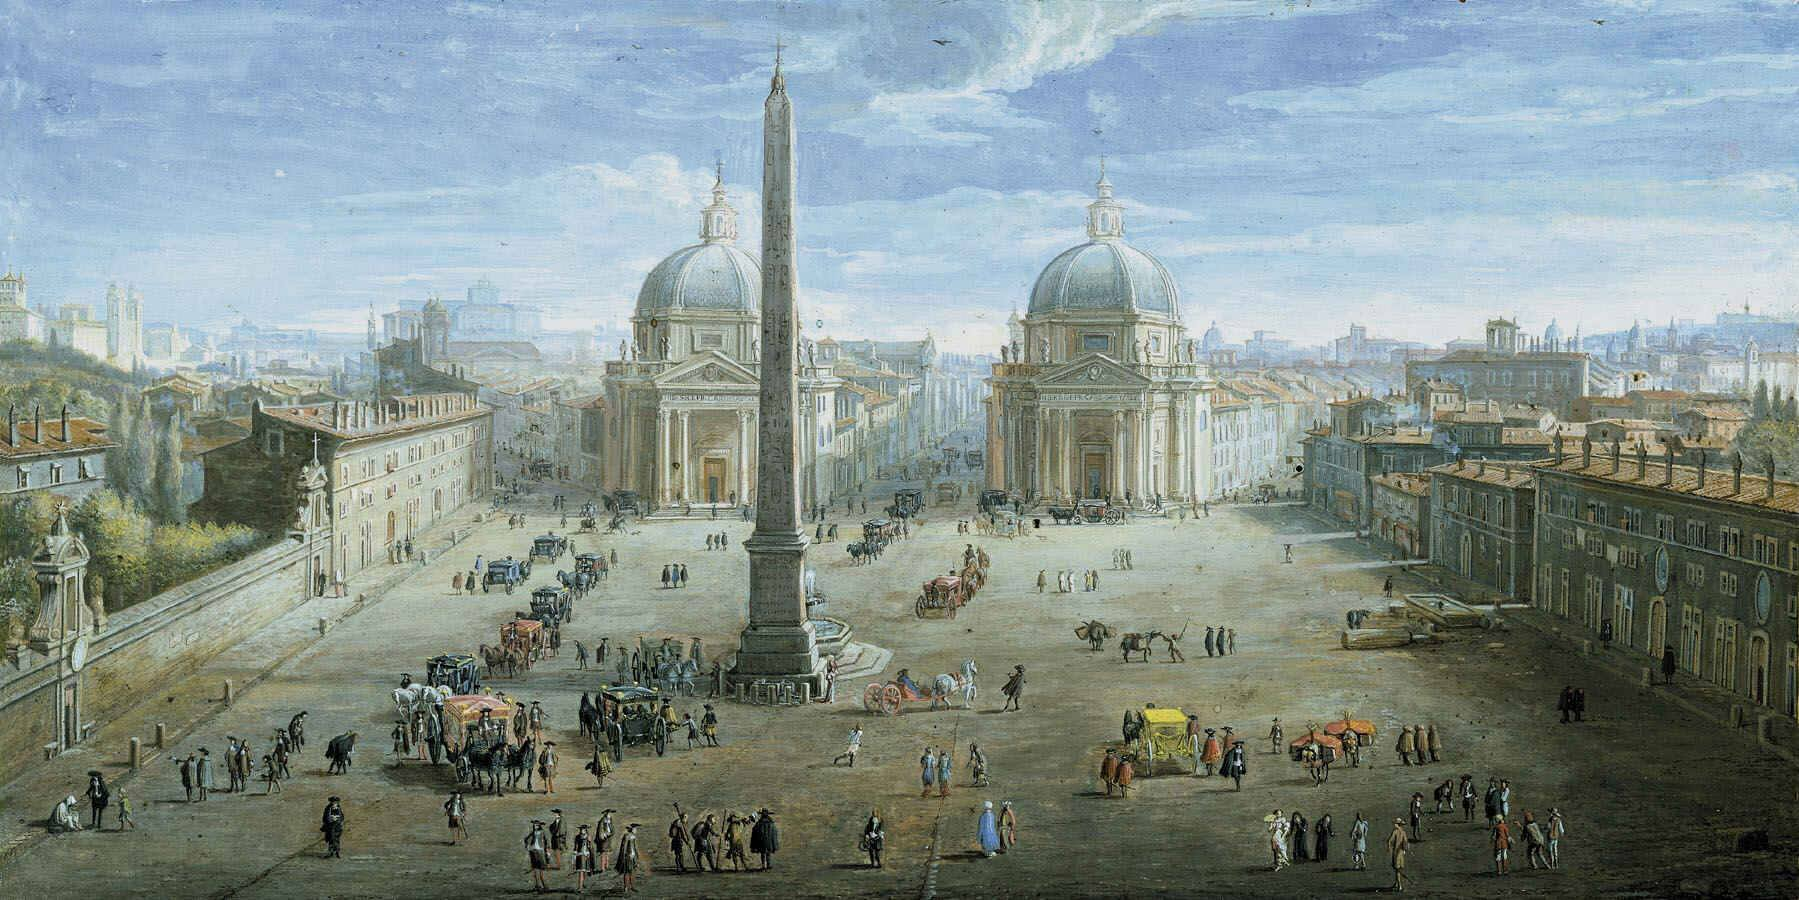
\includegraphics[width=1\textwidth]{/Users/Pancratii/GitHub/phd/Sections/Projeto_de_Pesquisa_2023-03-18_Teste/Pictures/popolo.jpeg} 
	            \captionsetup{labelfont=bf}
	            \caption{Vista da \textit{Piazza del Popolo}, em Roma, por Caspar Van Wittel (1652–1736). \textbf{Fonte:} Wikimedia Commons / Sotherby's (coleção privada).}
	            \label{fig:popolo}
            \end{figure}   

            Discorramos rapidamente sobre a ideia de \textit{forma} e traçado. Traçado é o particípio do verbo traçar, \textit{i.e.,} desenhar traços, riscar, sendo o ato ou efeito desse mesmo verbo, resultando, portando, em um `conjunto de traços', ou, no nosso caso, no `desenho que representa uma estrutura arquitetônica ou urbanística', o que é equivalente a dizer `planta', `projeto', ou, para usar um termo mais antigo, `traça' (PRIBERAM, TRAÇADO, 2023). Na língua rústica do latim, `tracto' que dizer `traçar sulcos', e `tractus' é a `delimitação por meio de traços; região, lugar, quarteirão' (FARIA, 1962, p. 1010). Penso que não haja melhor definição que essa: `delimitação por meio de traços' – que corrobora com a ideia de trajetória de estrada ou mesmo linha férrea (PRIBERAM, TRAÇADO, 2023). \textit{Forma,} porém, é um termo mais complexo.

            \begin{figure}
	            \centering
	            \includegraphics[width=1\textwidth]{/Users/Pancratii/GitHub/phd/Sections/Projeto_de_Pesquisa_2023-03-18_Teste/Pictures/nolli_popolo.png}
	            \captionsetup{labelfont=bf}
	            \caption{\textit{La nuova topografia di Roma} (detalhe), de Gianbattista Nolli (1701-1756), com a \textit{Piazza del Popolo} ao norte. \textbf{Fonte:} UC Berkeley Library.}
	            \label{fig:nolli_popolo}
            \end{figure} 

            \textit{Forma} é a `configuração das coisas na parte exterior', o que é equivalente a `feitio' e `formato' (PRIMERAM, FORMA, 2023). No latim, a coisa complica um pouco, com \textit{`forma'} querendo dizer `fôrma' (que em português é um `molde sobre o qual ou dentro do qual se coloca alguma substância fluida, que toma o feitio desse molde'), ou `todo objeto feito na fôrma'; pode, de fato, ser entendida como `desenho, modelo, planta', mas também pode ser entendida como `tipo ideal', ou ainda como `conformação, configuração, constituição' (FARIA, 1962, p. 407). E, se formos para o campo da filosofia, aí é que a confusão aumenta, pois temos um `sentido filosófico e particularmente metafísico', um `sentido lógico', outro `epistemológico', um metodológico', e, por fim, ainda um `sentido estético' (MORA, 2001b, p. 1126) – e, portanto, a ideia de \textit{`forma'} escapa-nos neste momento.

            Desse modo, na presente pesquisa, meu foco se direciona ao `traçado urbano' e não à \textit{`forma} urbana'. No entanto, é necessário esclarecer que o termo `traçado urbano', por sua vez, pode ter mais de uma acepção. Se pensarmos que a \textit{`forma'} da cidade é constituída por seu aspecto tridimensional,
                \footnote[6]{Aqui faço minhas as palavras de José Lamas (2010, pp. 41 e 48), ao dizer que a forma urbana corresponde "ao meio urbano como arquitectura, ou seja, um conjunto de objectos arquitectónicos ligados entre si por relações espaciais" e que é "a materialização no espaço da resposta a um contexto preciso".} 
            com suas edificações e demais estruturas, podemos deduzir que o `traçado' é a marca deixada no solo por essa \textit{`forma'}. Logo, o `traçado' da cidade seria o sulco resultante dos limites dos lotes e quarteirões e dos contornos edificados (que, não raro, definem o próprio desenho das vias, por meio da conjunção de fachadas).
                \footnote[7]{Note-se que, diferente do que atualmente é lugar comum, o que definia o que era ou não a rua, seu limite, seu contorno, seu espaço, era precisamente a fachada da edificação, que imprime essa linha ao mesmo tempo imaginária e real no solo, diferente do que ocorre hoje. Hoje, o lugar comum é aquele de que o que define a via é o meio-fio — ou o limite do lote, que não coincide com a implantação da edificação, com a marca que a mesma deixa sobre o solo. E isso é fruto da desvinculação entre edificação e lote, entre os limites da edificação e os limites do lote. Mas, se olharmos para nosso passado urbano, veremos algo bem diferente. Basta olharmos uma pintura de Caspar Van Wittel da \textit{Piazza Navona} em Roma e veremos como a praça já era muitíssimo bem definida (pelas edificações), mesmo sem qualquer indício de calçamento, e muito menos de meio-fio.} 

            No entanto, aqui, pretendo que o termo `traçado urbano' tome uma ênfase particular. Isso não exclui o sentido aludido acima, posto que tratarei de contornos edificados, lotes e quarteirões ao falar de `traçado urbano' ao longo desta tese – porém serei específico quando o fizer. Desse modo, a ênfase que quero dar é a de `traçado urbano' enquanto sinônimo de `espaço público', tanto na definição de Vitor Oliveira (2016)
                \footnote[8]{\textit{`The public spaces system of a city includes (...) the open spaces for movement, which we designate, in a simplified way, as streets, (...) [and] also the open spaces for permanence, which we designate as squares and gardens.'} (OLIVEIRA, 2016, p. 17).} 
            quanto, particularmente, na visão de Huimin Ji e Wowo Ding (2021) – que trazem uma releitura contemporânea de Gianbattista Nolli (\autoref{fig:nolli_popolo}). Assim, o termo `traçado urbano' se relaciona com as vias, praças e áreas públicas de edificações – espaços com acesso franqueado ao público. Percursos, nós e polos abertos e fechados, cobertos e descobertos, percorríveis em um único plano contínuo: o plano do solo.
                \footnote[9]{Podemos chamar esse plano de `térreo', ainda que ele comporte variações de altitude e inclinação; porém a ideia é a de que esse é o "plano-base" da cidade, a partir do qual se desenvolvem as edificações, para cima ou para baixo.} 
            Por vias podemos tomar percursos como ruas, calçadões, \textit{woonerfs}, escadarias e alamedas e espaços abertos de parques urbanos (excluídos os maciços vegetais), levando em conta a apropriação dos elementos contidos nesses espaços, como ocorre com os canteiros (HANNES, 2016);
                \footnote[10]{Canteiros que, atualmente, são considerados algo à parte, algo que não é inerente à via, mas que a define e delimita, posto que, para boa parte das prefeituras, o que determina o limite da via não é o \textit{continuum} das fachadas das edificações, senão o limite dos lotes (muros), as guias de meio-fio e os canteiros: elementos definidores da rua que não mais estão destinados a um uso comum.} 
            bem como estacionamentos descobertos, além de rodovias e ferrovias (posto que servem de passagem para pessoas e suas mercadorias e que possuem uma marca sobre o solo que se relaciona com o desenho do restante da cidade). Por praças, podemos entender tanto a clássica praça, espaço aberto de dimensões superiores à da rua, o largo, o \textit{pocket park}, desde que descobertos – exceção feita aos \textit{`annodamenti'} (dos quais se tratará no momento oportuno), que ficam em uma situação ambígua de área pública de edificação e praça. E as áreas públicas de edificações podem ser exemplificadas pelas naves das igrejas, pelas platéias dos teatros e pelos halls, corredores, pátios e praças cobertas dos  edifícios públicos, galerias comerciais, mercados e \textit{shopping centers}.

            Dito isso, reforço que: em relação às `formas' edificadas, conhecemos os motivos da crise atual  – e podemos mesmo ir mais a fundo, entendendo as dinâmicas inerentes aos materiais, à economia, às tendências ditadas de tempos em tempos pelas publicações e sua relação com o design de outras áreas. Temos ideia de como estabelecer um liame com o passado, inclusive com exemplos projetuais – e, quando não (como no caso do Brasil), temos um método para `ler' as pré-existências edificadas e, a partir delas, deduzir o \textit{tipo} edilício de um território, de modo a ter o balizador para novas edificações. E nisso reside a força da escola italiana de tipomorfologia urbana. Todavia, mais uma vez: se podemos sabemos como obter respostas em relação à \textit{forma} da cidade, o mesmo não se dá em relação ao seu traçado.

            \section{Rendimento}%conteúdo anterior [reprovado 10 OUT 2023]
            
            \textit{Rendimento}, ``grau de coerência [de algo] com o contexto'' (Maffei, 2003, p. 82, tradução nossa).  Até minha dissertação, pude levantar duas acepções para o termo: uma, o \textit{`rendimento} edilício', e outra, o \textit{`rendimento'} territorial. A primeira é uma dialética entre a ação do homem e uma reação do ambiente (antrópico) no qual ele está inserido (Caniggia e Maffei, 2008, p. 52). A segunda é a medida com que um território pode ser utilizado pelo homem (Carlotti, 1995, p. 19). Dessas duas escalas, pude deduzir uma nova acepção, que intitulei \textit{`rendimento} urbano', ou seja, ``a coerência intrínseca entre o traçado da forma urbana e o contexto natural'' (Costa, 2020, p. 52). Assim, tomando esse ponto de partida, faz-se necessário destrinchar alguns conceitos e definições.

            A proposição inicial da minha tese é a de que `é possível projetar traçados urbanos morfologicamente adequados ao contexto'. Mais que isso, tais traçados não são traçados `adaptados', com uma forma concebida \textit{a priori}, que só depois é confrontada com a realidade e então deformada por ela – como o seria um \textit{grid}, uma matriz de linhas ortogonais. Ao contrário, tais traçados devem ser adequados ao contexto desde sua concepção. Ou seja, o contexto vem antes. É ele que direciona o projeto. Ou melhor, o processo de projeto parte da consideração de suas formas, e, desse modo, o contexto dá a \textit{forma} do traçado urbano. Nesse sentido, vale a pena esmiuçar melhor o que quero dizer com termos como `forma', `traçado', `contexto', `morfologicamente adequado', e outros termos relacionados como `território' e `paisagem' – quero dizer, é necessário mostrar suas acepções e de quais autores extraio tais conceitos.

            \section{Traçado urbano}%conteúdo anterior [reprovado 10 OUT 2023]
                \subsection{Forma urbana}
                \subsection{Elementos antrópicos do traçado: percursos, nós e polos}
                \subsection{Estruturas naturais subjacentes ao traçado}
                    \subsubsection*{Definições de paisagem e território}
                Para Giuseppe Strappa (2014, p. 19, tradução nossa), %https://issuu.com/giuseppestrappa/docs/strappa_diadi_mediterranee_2014
                    ``o território é um modo de olhar o mundo (...), [de ler] a forma das coisas (dos solos, dos percursos, dos assentamentos) para compreender sua estrutura, entender suas origens [e] possíveis transformações''. O território, continua, ``é o conjunto inscindível de solo e trabalho do homem que o habita e transforma, [em suma,] é arquitetura.'' O termo `paisagem', portanto, ``é o aspecto reconhecível da sua estrutura, a sua forma [, que contém um conjunto de contribuições].'' Ou seja, a `paisagem' para Strappa é a forma do território. Um não contém o outro, mas um é a manifestação do outro.\footnote[11]{\textit{``In architettura il territorio è un modo di guardare il mondo. Di leggere, cioè, la forma delle cose (dei suoli, dei percorsi, degli insediamenti) per afferrarne la struttura, capirne le origini, le possibili trasformazioni. Il territorio è l'insieme inscindibile di suolo e lavoro dell'uomo che lo abita e lo trasforma, è architettura. Il termine `paesaggio' è l'aspetto riconoscibile della sua struttura, la sua forma che contiene un insieme di contributi''} (Strappa, 2014, p. 19).}

                    Em uma nota de rodapé, Strappa (2019, \textit{s.p.}) escreve ainda: %http://www.giuseppestrappa.it/wp-content/uploads/2019/10/cap.-10-territorio-per-il-corso.pdf http://www.giuseppestrappa.it/?p=8355
                    \begin{quotation}
                        ``\emph{Land-scape} significa em inglês `modelagem da terra', com ênfase no aspecto natural do ambiente cognitivo com o qual o termo está associado. Ele se opõe ao termo italiano \emph{`paesaggio'} (francês \emph{`paysage'}, espanhol \emph{`paisaje'}), associado ao termo \emph{`paese'} e, portanto, ao latim \emph{`pagus'}, que significa vila, reconhecendo, de maneira concisa, uma relação de solidariedade entre a terra e o assentamento humano. Portanto, a paisagem como expressão cultural está ligada ao espaço habitado, à cooperação entre recursos naturais e artificiais, às transformações que interpretam a forma de picos orográficos, vales, planícies e sua capacidade de se tornar um ambiente construído. Em resumo, [paisagem] é o aspecto visível do território, a expressão concisa de sua estrutura'' (tradução nossa).\footnote[12]{\textit{``Land-scape'' means in English ``modelling of the earth'', with an emphasis on the natural aspect of the cognitive environment the term is associated with. It is opposed to the Italian term ``paesaggio'' (French ``paysage'', Spanish ``paisaje'') associated with the term ``paese'' and hence to the Latin ``pagus'' meaning village, acknowledging, in a concise manner, a relationship of solidarity between the land and human settlement.Therefore, the landscape as a cultural expression is linked to the inhabited space, to the cooperation between natural and artificial resources, to the transformations that interpret the form of orographic peaks, valleys, plains and their ability to become a built environment. In short, it is the territory’s visible aspect, the concise expression of its structure''} (Strappa, 2019, \textit{s.p.}).}
                    \end{quotation}

                \subsection{Relações entre traçado urbano, parcelamento rural e áreas não-antropizadas}
                
                Não é possível reconhecer o traçado urbano como um mero objeto autônomo, sem relação com o solo sobre o qual se assenta, solo esse que também é subjacente ao território que circunda esse traçado. Desse modo, o traçado urbano deve ser entendido dentro do \textit{framework} dado pelo território, ambos sustentados por um solo com características naturais peculiares a cada lugar, formando, assim, uma paisagem só.\footnote[13]{Para Strappa (2013, \textit{s.p.}), a noção de território deriva do nexo entre a ideia de contexto natural e transformações antrópicas desse mesmo contexto natural, o que o faz entender a paisagem como aspecto visível de uma estrutura de relações que conecta os diversos graus e escalas do universo construído dentro da noção de organismo. Escreve: \textit{``Il concetto di territorio deriva dal nesso che lega l’idea di suolo naturale a quella delle trasformazioni artificiali operate dall’uomo nel processo di antropizzazione (trasformazione abitativa e produttiva) del suolo stesso. Noi cogliamo questo processo attraverso momentanei stati di equilibrio che  restituiscono un’idea discreta di una sequenza storica che è, invece, flusso continuo di modificazioni e rivolgimenti.
                Per questo non è comprensibile il senso storico-processuale di un organismo urbano o di un sistema di percorrenze, se non si colloca la loro formazione all’interno di un rapporto di necessità con l’insieme delle relazioni instaurate nel tempo e nello spazio entro il proprio intorno territoriale. Questa forma del territorio antropizzato non é che l’aspetto visibile di una struttura di relazioni che lega nella nozione di organismo i diversi gradi scalari del costruito e che indicheremo col termine `paesaggio'.''} Essa definição mesma de `paisagem' serve para indicar o que é o contexto antrópico.}

            \section{\textit{Modus faciendi} atual}
                \subsection{Manuais, guias e leis de parcelamento do solo}
                \subsection{Entrevistas sobre princípios que norteiam o desenho dos traçados}
                \subsection{Rendimento econômico}
            \section{Morfoadequabilidade: uma nova definição} %Ver se não fica melhor antes da seção sobre o modus faciendi atual.

        \chapter[Maringá: um novo estudo de caso]{um novo estudo de caso sobre Maringá}

        \begin{itemize} %O que analisar no estudo de caso de Maringá
            \item A relação entre território (CTNP) e traçado (esqueleto) em Maringá
            \item O traçado do Vieira (parâmetro de qualidade)
            \item As expansões urbanas (o modo como as expansões urbanas são feitas)
        \end{itemize}

        O traçado de Maringá é digno de nota não apenas por sua conformação, mas pelo fato de ter conseguido uma configuração ímpar dentro das suas condicionantes, e mantendo um rendimento econômico adequado para a Companhia. É verdade que, olhando a topografia, o traçado de Maringá poderia ter uma configuração totalmente diferente. No entanto, dentro do seu ideário, e baseando-se na ferrovia como ponto de partida, o traçado projetado por Vieira assumiu uma configuração bastante adequada ao contexto natural. A ferrovia foi o pontapé inicial, sendo o elemento balizador do território enquanto framework, território esse desenvolvido a partir das estruturas naturais, ao menos em larga escala, por meio do desenho Waldhufendorf do parcelamento rural. E Vieira, aproveitando esse elemento estruturador (a ferrovia), apoiou o restante do traçado sobre as estruturas naturais circunstantes à ferrovia e em sintonia com as estruturas antrópicas do território – como estradas rurais e carreadores – encaixando o traçado geometrizado em uma topografia orgânica por meio da utilização de curvas e retas.

        \begin{center}
        . . . . .
        \end{center} 

        Como Vieira nunca esteve em Maringá, é de se suspeitar que o material que ele recebeu foi o levantamento topográfico da gleba destinada pela Companhia para a cidade de Maringá. Note-se que era prática da Companhia separar glebas para suas cidades e patrimônios dentro do parcelamento rural do território pertencente à Companhia. E, nesse sentido, apesar de não haver (ao menos não em meu conhecimento até o momento) nenhum mapa em que conste uma `gleba Maringá' ou algo semelhante, é possível notar no Anteprojeto para Maringá a definição das curvas de nível e de tracejados que as delimitam, corroborando com a hipótese(*) levantada. Desse modo, não é de admirar que Vieira tenha inserido vias que continuam para além dos limites do seu projeto, como fios desencapados à espera de continuação, e que, eventualmente, conflitam com o traçado das estradas rurais da Companhia – note-se, por exemplo, a avenida curva a sudoeste do Anteprojeto que não perfaz o \textit{offset} da estrada Cleópatra: aqui a avenida segue de maneira pormenorizada a cumeada do promontório, enquanto a estrada (como se pode ver em outro mapa) apenas se aproxima da cumeada, mas que não se apoia necessariamente nesta, nem nos pontos de relevo mais suave, seguindo uma linha reta desenhada a partir de uma linha de força que conecta o início e o fim do promontório.

        \chapter[A escolha de uma solução]{artefato a desenvolver}

        [09OUT2023 14:40 SCADA] Na busca por uma solução, nem mesmo Waldheim (2016) mostra algo que congregue o desenvolvimento de traçados urbanos com a topografia. Topografia que, segundo ele (p. ?), é aquilo que une arquitetura, urbanismo e paisagem (architecture, urban design and landscape). Ele mostra parques, e o modo como esses parques interagem na dinâmica das cidades, mas não a morfologia das cidades em si.
        O que proponho aqui, por outro lado, é uma 'nova abordagem' em relação à forma dos traçados urbanos, particularmente para as novas áreas urbanas. Novas áreas urbanas essas que não precisam necessariamente estar vinculadas à expansão urbana, mas podem – e devem – estar atreladas, por exemplo, ao preenchimento dos vazios urbanos presentes em nossas cidades e que podem ser remanejados com uma solução morfoadequada que aguegue traçados urbanos e \textit{landscape urbanism}. (Cf. Waterfront Toronto).

    \part[Desenvolvimento]{Desenvolvimento}

        \chapter[Protocolo]{Protocolo de desenvolvimento do artefato}

        \chapter[O projeto de traçados hipotéticos]{Pilotos}
            
            \section{Projeto hipotético sobre \textit{tabula rasa} (\textit{land readjustment}/Dissertação)}
            \section{Projeto hipotético sobre pré-existências (Diretrizes Viárias/PIBIC)}
            \section{Projeto hipotético sobre parcelamento rural}

        \chapter[Diretrizes projetuais]{artefato – versão inicial}

    \part[Avaliação]{Avaliação}

        \chapter[Comparativo com existente]{estudo de caso}

        \chapter[Grupos focais e \textit{feedback}]{}

        \chapter[Diretrizes projetuais]{artefato – versão refinada}

            \section[Comunicação do artefato aos \textit{stakeholders}]{title}

    %\backmatter % Seção de pós-texto (bibliografia, apêndices, anexos, etc.)            

    \part*{}

        \chapter*{Conclusão}
        \addcontentsline{toc}{chapter}{Conclusão}

        \chapter*{Referências}
        \addcontentsline{toc}{chapter}{Referências}

            \bibliography{bibliografia} % Arquivo .bib com as referências bibliográficas
            % Adicione apêndices e anexos conforme necessário

        \chapter*{Anexos}
        \addcontentsline{toc}{chapter}{Anexos}

\end{document}
